% Chapter 2
\chapter{Traditional RGB-D Cameras Calibration} % Main chapter title
\label{chapterTraditionalCalibration} % For referencing the chapter elsewhere, use \ref{sens_introduction} 

\section{Pinhole Camera}
\label{sectionPinholeCamera}
%%%%%%%%%%%%%%%%%%%%%%%%%%%%%%%%%%%%%%%%%%%%%%%%%%%%%
%%%%%%%%%%                                                                                                   %%%%%%%%%%
%%%%%%%%%%      1. Intrinsic, introduce camera model from 3D to 2D:         %%%%%%%%%%%
%%%%%%%%%%                 (X^c, Y^c, Z^c) --> (R, C)                                          %%%%%%%%%%%
%%%%%%%%%%%%%%%%%%%%%%%%%%%%%%%%%%%%%%%%%%%%%%%%%%%%%%
\indent
A pinhole camera is a simple optical imaging device in the shape of a closed box or chamber. A pinhole camera is completely dark on all the other sides of the box including the side where the pin-hole is created. Fig.~\ref{PinholeCameraFigure} shows an inspection of a pinhole camera. In its front is a pin-hole that help create an image of the outside space on the back side of the box. When the shutter is opened, the light shines through the pin-hole and imprint an image onto a sensor (or photographic paper, or film) placed at the back side of the box. In order to analyze parameters like focal distance, field of view, etc., pinhole camera has its own three dimensional space (noted as \(X^\text{c}\), \(Y^\text{c}\), and \(Z^\text{c}\)). Note that, according to Cartesian Coordinates \enquote{right hand} principle, the camera is looking down the negative of \(Z^\text{c}\)-axis, given \(X^\text{c}\)\(Y^\text{c}\) directions as shown in the figure. Its focal length of the pinhole camera is the distance on the \(Z^c\)-axis, between the pinhole at the front of the camera and the paper or film at the back of the camera.\par
%
\begin{figure}[!b]
\centering
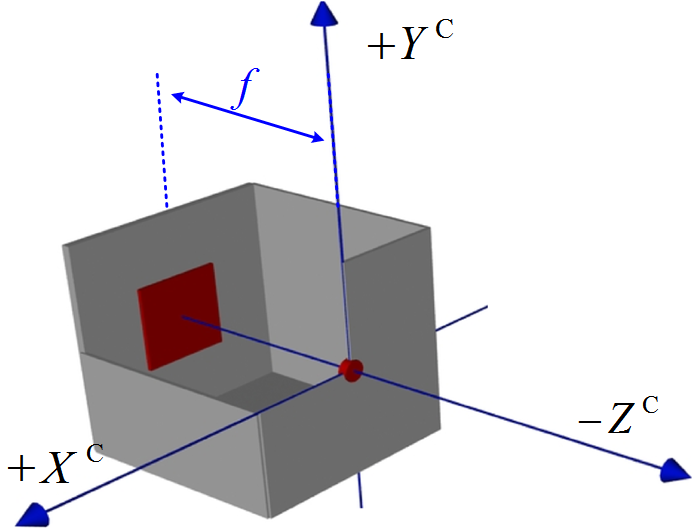
\includegraphics[width=0.45\textwidth]{PinholeCameraFigure}
\caption{The Pinhole Camera Inspection}
\label{PinholeCameraFigure}
\end{figure}%
%
\begin{figure}[!h]
\centering
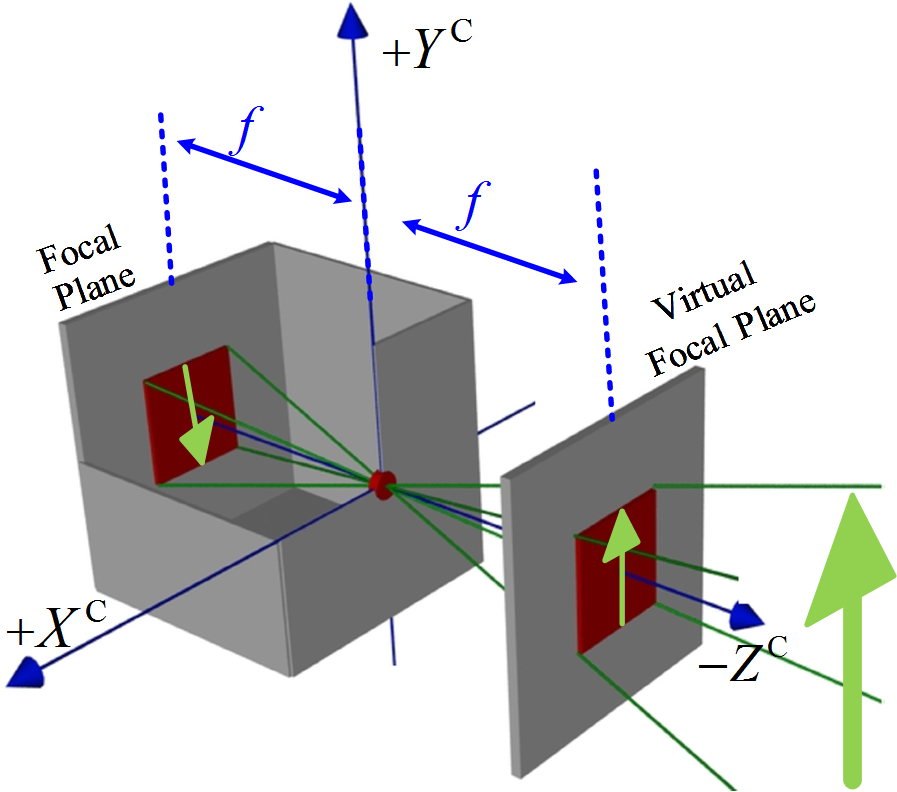
\includegraphics[width=0.5\textwidth]{PinHoleVirtualFocalPlane}
\caption{Virtual Focal Plane of a Pinhole Camera}
\label{PinHoleVirtualFocalPlane}
\end{figure}%
%
%
Pinhole cameras are characterized by the fact that they do not have a lens. It rely on the fact that light travels in straight lines, which is a principle called the rectilinear theory of light. This makes the image appear upside down in the camera, as shown in fig.~\ref{PinHoleVirtualFocalPlane}. Tracing the corners of the camera sensor through the pin hole, those dark green lines show the limits of the field of view in 3D coordinate space. The back side plane of the pinhole camera, which is behind the origin at a positive \(Z^c\)-axis and also where our sensor sits, is also called the focal plane. It is not intuitive, nor convenient for mathematical analysis that the images on the focal plane are always upside down. So a virtual focal plane is defined created in front of the pinhole on the negative \(Z^c\)-axis, which is equal distant from the focal point (pin hole) as the actual focal plane is behind. Notice that the limits of the field of view intersect with the virtual focal plane at the four corners of the up-right image just as they disseminate from the four corners of the sensor at the real focal plane.

\begin{figure}[b]
\centering
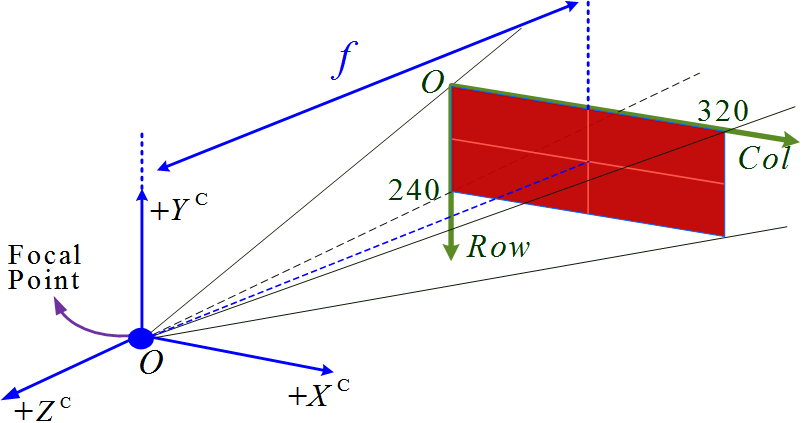
\includegraphics[width=0.65\textwidth]{CommonPinholeCameraModel}
\caption{Common Pinhole Camera Model}
\label{CommonPinholeCameraModel}
\end{figure}%
%

With the virtual focal plane, the camera body with the real focal plane could be removed. And the rest parts in front of the the camera body, the focal point and the virtual focal plane together, form the most common pinhole camera model. In order to employ this model for 3D analyzing points inside the camera's field of view based on 2D image, the most prior step is to define the relationship between points in 3D camera space and the 2D image coordinates row and column of the corresponding captured image. As shown in fig.~\ref{CommonPinholeCameraModel}, only the sensor (in color red) is visible at the virtual focal plane. The focal point is right at the origin of the camera 3D space coordinates, from where to the sensor has the vertical distance of \(f\), the focal distance. The 2D image coordinates are in dark green, where its origin is sitting at the up-left corner of the sensor. Taking the PrimeSense camera, whose RGB and Depth sensor share the pixel height and width 240*320. As long as both of the camera 3D space and image 2D space are defined, the next step is the determine the determine their relationship. Note that, the range of image should be either ([0:239], [0:319]) or ([1:240], [1:320]).
%
\begin{figure}[b]
\centering
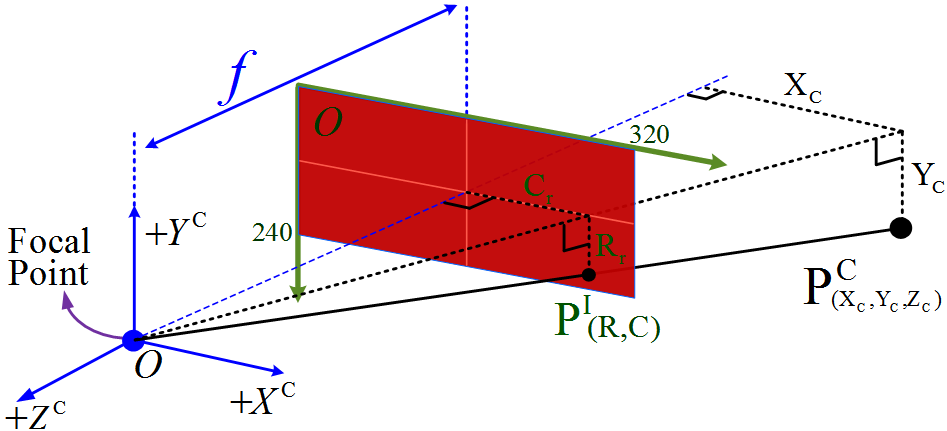
\includegraphics[width=0.9\textwidth]{RelationshipCameraToImage}
\caption{Mapping from Camera Space to Image Space}
\label{RelationshipCameraToImage}
\end{figure}%
%

Select a random object point \(\text{P}^\text{C}\) in the camera space located at camera 3D coordinates (\(\text{X}_\text{C}\), \(\text{Y}_\text{C}\), \(\text{Z}_\text{C}\)). A line passing both of the point \(\text{P}^\text{C}\) and the focal point intersects with the virtual focal plane at \(\text{P}^\text{I}\), with its image 2D coordinates (R, C). To determine the mapping function, we can start a the proportional relationship. As shown in fig.~\ref{RelationshipCameraToImage}, the center point in the image coordinates, which is usually called \enquote{principle point}, could be determine by column of half-width and row of half-height. Concretely, the principle point (\(\text{R}_\text{h}\), \(\text{C}_\text{h}\)) is either (119.5, 159.5) if range is ([0:239], [0:319]), or (120, 320) if range is ([1:240], [1:320]). So, we could get the relative row and column distance of  \(\text{R}_\text{r}\) and \(\text{C}_\text{r}\)) by eqn.~\ref{relativeCRforProportional}.
%
\begin{equation}
\begin{aligned}
\text{R}_\text{r} = \text{R} - \text{R}_\text{h}%
\\%
\text{C}_\text{r} = \text{C} - \text{C}_\text{h}%
\end{aligned}
\label{relativeCRforProportional}
\end{equation}%
%
Based on by triangulation, it is straight forward to tell the proportional relationship between \(f\)/\(\text{Z}_\text{C}\) and \(\text{C}_\text{r}\)/\(\text{X}_\text{C}\), \(\text{R}_\text{r}\)/\(\text{Y}_\text{C}\). Thus we get eqn.~\ref{twoDRelativeFromCamToIm}.
%
\begin{equation}
\left[ \begin{array}{c} \text{C}_\text{r} \\ \text{R}_\text{r} \end{array} \right] %
= f %
\left[ \begin{array}{c} \text{X}_\text{C}/\text{Z}_\text{C} \\ \text{Y}_\text{C}/\text{Z}_\text{C} \end{array} \right]%
\label{twoDRelativeFromCamToIm}
\end{equation}
\noindent
And by changing the relative distance \(\text{R}_\text{r}\text{C}_\text{r}\) back to the 2D image coordinates (R, C), then eqn.~\ref{twoDRelativeFromCamToIm} will be written as
%
\begin{equation}
\left[ \begin{array}{c} \text{C} \\ \text{R} \end{array} \right] %
= f %
\left[ \begin{array}{c} \text{X}_\text{C}/\text{Z}_\text{C} \\ \text{Y}_\text{C}/\text{Z}_\text{C} \end{array} \right]%
+
\left[ \begin{array}{c}  \text{C}_\text{h} \\  \text{R}_\text{h} \end{array} \right] ,%
\label{linearRelationFromCamToIm}
\end{equation}
\noindent
if written in homogeneous coordinates, we will get eqn.~\ref{HomoProportionalRelationFromCamToIm}.
\begin{equation}
%
\text{Z}_\text{C} \left[ \begin{array}{c} \text{C} \\ \text{R} \\ 1 \end{array} \right] %
= %
\left[ \begin{array}{c} f\text{X}_\text{C} \\ f\text{Y}_\text{C} \\ \text{Z}_\text{C} \end{array} \right]%
+
\left[ \begin{array}{c}  \text{Z}_\text{C}\text{C}_\text{h} \\  \text{Z}_\text{C}\text{R}_\text{h} \\ 0\end{array} \right] %
=  \begin{bmatrix} f & 0 &  \text{C}_\text{h}  \\ 0 & f & \text{R}_\text{h} \\ 0 & 0 & 1 \end{bmatrix}%
\left[ \begin{array}{c} \text{X}_\text{C} \\ \text{Y}_\text{C} \\ \text{Z}_\text{C} \end{array} \right]%
\label{HomoProportionalRelationFromCamToIm}
\end{equation}%
%
\\\indent
Till Now, we haven't consider the units translation between the camera 3D space the image 2D space. The random object point \(\text{P}^\text{C}\)'s mapping point \(\text{P}^\text{I}\) (R, C) on the image space is expressed in millimeters (or inches). Since it is necessary to express the image space coordinates (R, C) in pixels, we need to find out the resolution of the sensor in pixels/millimeter. Considering that, the pixels are not necessarily be square-shaped, we assume they are rectangle-shaped with resolution  $\alpha_c$ and \(\alpha_r\) pixels/millimeter in the \(Col\) and \(Row\) direction respectively. Therefore, to express \(\text{P}^\text{I}\) in pixels, its C and R coordinates should be multiplied by \(\alpha_c\) and \(\alpha_r\) respectively.
%
\begin{equation}
\left[ \begin{array}{c} \text{Z}_\text{C} \text{C} \\ \text{Z}_\text{C} \text{R} \\ \text{Z}_\text{C}  \end{array} \right] %
= %
\left[ \begin{array}{c} f\alpha_c\text{X}_\text{C} \\ f\alpha_r\text{Y}_\text{C} \\ \text{Z}_\text{C} \end{array} \right]%
+
\left[ \begin{array}{c}  \text{Z}_\text{C}\alpha_c\text{C}_\text{h} \\ \text{Z}_\text{C}\alpha_r\text{R}_\text{h} \\ 0 \end{array} \right] %
=  \begin{bmatrix} \alpha_cf & 0 &  \alpha_c\text{C}_\text{h}  \\ 0 & \alpha_rf & \alpha_r\text{R}_\text{h} \\ 0 & 0 & 1 \end{bmatrix}%
\left[ \begin{array}{c} \text{X}_\text{C} \\ \text{Y}_\text{C} \\ \text{Z}_\text{C} \end{array} \right]%
= K\text{P}^\text{C}
\label{HomoProportionalFromCamToImInPixels}
\end{equation}%

\noindent
Note that \(K\) only depends on the intrinsic camera parameters like its focal length, resolution in pixels, and sensor's width and height. Thus, the mapping matrix \(K\) is also called a camera's intrinsic matrix. Considering that the pixels might be parallelogram-shaped instead of rigid rectangle-shaped (when the image coordinate axis \(Row\) and \(Col\) are not orthogonal to each other), usually \(K\) has a skew parameter \(s\), given by

\begin{equation}
K%
=  \begin{bmatrix} 
f_c & s & t_c \\
 0 & f_r & t_r \\
 0 & 0 & 1 \end{bmatrix}%
\label{intrinsicKmatrix}
\end{equation} , %
\noindent
where \(f_c = \alpha_cf\) and \(f_r = \alpha_rf\) are the focal length in pixels on the \(Col\) and \(Row\) directions respectively,  \(t_c = \alpha_c\text{R}_\text{h}\) and \(t_r = \alpha_r\text{R}_\text{h}\) are the translation parameters that help move the origin of image coordinate to the principle point.\\

%%%%%%%%%%%%%%%%%%%%%%%%%%%%%%%%%%%%%%%%%%%%%%%%%%%%%
%%%%%%%%%%                                                                                                   %%%%%%%%%%
%%%%%%%%%%      2. Extrinsic, (X^w, Y^w, Z^w) --> (X^c, Y^c, Z^c)          %%%%%%%%%%%
%%%%%%%%%%                                                                                                    %%%%%%%%%%%
%%%%%%%%%%%%%%%%%%%%%%%%%%%%%%%%%%%%%%%%%%%%%%%%%%%%%%

Now we have \(K\), which helps map between camera 3D space and image 2D space. But we are still not able to employ it yet. The camera 3D space is respect to the camera sensor only. Neither can we directly tell the camera 3D coordinates of an object point, nor can we assign it. All we can do is to use the camera space as an intermediate between the image coordinates and world coordinates, which we could assign by ourselves.
%
\begin{figure}[!t]
\centering
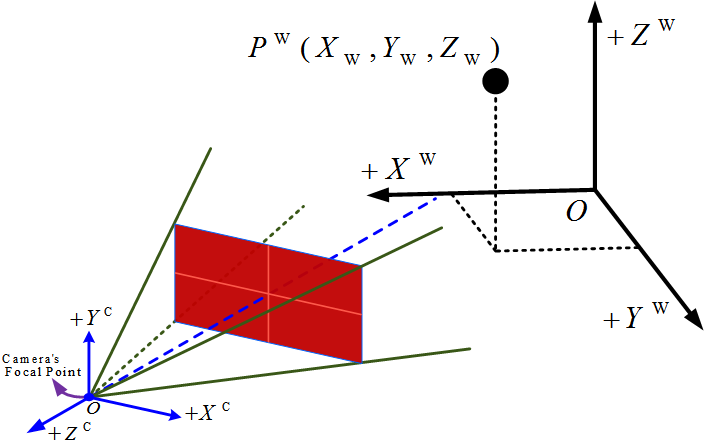
\includegraphics[width=0.65\textwidth]{FromWorldToCameraSpace}
\caption{Pinhole Camera in World Space}
\label{FromWorldToCameraSpace}
\end{figure}%
%

Fig.~\ref{FromWorldToCameraSpace} shows a pinhole camera observing an arbitrary object point P in the world  space. We assign the world coordinates so that the object point has world space coordinates \(P^W(X_w, \, Y_w, \, Z_w)\). Although the world space and camera space are two different spaces, we could easily transform between each other through rotation and translation, as long as both of the spaces are using rigid Cartesian Coordinates. With a standard rotation matrix \(R_{3*3}\) and a translation matrix \(T_{3*1}\)
%
\begin{equation}
R_{3*3}%
=  \begin{bmatrix} 
r_{11} & r_{12} & r_{13} \\
r_{21} & r_{22} & r_{23} \\
r_{31} & r_{32} & r_{33}
 \end{bmatrix}%
, \, \, 
T_{3*1}%
=  \begin{bmatrix} 
t_{1} \\
t_{2} \\
t_{3}
 \end{bmatrix} ,%
\label{rotationTranslationMatrixRT}
\end{equation}%
%
we can get the transformation matrix \([R_{3*3} \,\, T_{3*3}]\) from the world space to camera space, as shown in eqn.~\ref{mappingFromWorldToCameraSpace}.
%
\begin{equation}
\begin{bmatrix} 
X^{C} \\
Y^{C} \\
Z^{C}
 \end{bmatrix}%
=  R \begin{bmatrix} 
X^{W} \\
Y^{W} \\
Z^{W}
 \end{bmatrix}%
 + T
=
\begin{bmatrix} 
R_{3*3} & T_{3*1} \\
\end{bmatrix}%
 \begin{bmatrix} 
X^{W} \\
Y^{W} \\
Z^{W} \\
1
 \end{bmatrix}%
\label{mappingFromWorldToCameraSpace}
\end{equation}%
%
%%%% 2.5 Pinhole Camera Matrix (X^w, Y^w, Z^w) --> (X^c, Y^c, Z^c) --> (R, C)
%
%
The parameters that help map from world space to camera space depend on how we assign the world coordinates. Since none of them are from the camera even though they are belongs to an important part of camera calibration, usually the matrix \([R_{3*3} \,\, T_{3*3}]\) is called extrinsic camera matrix. With both of the extrinsic camera matrix (help map from world space to camera space) and the intrinsic camera matrix (help map from camera space to image space), we are now able to build the connection between the world space coordinates, which could be assigned by ourselves, and the image space \(Row\) and \(Column\), which are the streams we retrieved from the camera. To combine the intrinsic camera matrix and extrinsic camera matrix (combine eqn.~\ref{HomoProportionalFromCamToImInPixels} and eqn.~\ref{mappingFromWorldToCameraSpace}), we get 

\begin{equation}
Z^C\left[ \begin{array}{c} C \\ R \\ 1 \end{array} \right] %
=K \left[ \begin{array}{c} X^C \\ Y^C \\ Z^C\end{array} \right]%
=K\begin{bmatrix} R_{3*3} & T_{3*1} \end{bmatrix} \left[ \begin{array}{c} X^w \\ Y^w \\ Z^w \\ 1 \end{array} \right]%
=M \left[ \begin{array}{c} X^w \\ Y^w \\ Z^w \\ 1 \end{array} \right]%
%
\label{pinholeCameraMatrixCalculation}
\end{equation}%
%
\begin{equation}
M = K\begin{bmatrix} R_{3*3} & T_{3*1} \end{bmatrix}%
= \begin{bmatrix} 
m_{11} & m_{12} & m_{13} & m_{14} \\
m_{21} & m_{22} & m_{23} & m_{24} \\
m_{31} & m_{32} & m_{33} & m_{34} \\
\end{bmatrix} , %
\label{pinholeMatrix3x4M}
\end{equation}%
%
where \(M=K[R_{3*3} \,\, T_{3*1}]\), as written in eqn.~\ref{pinholeMatrix3x4M}. \par
%
Note that, although \(Z^C\) values can be retrieved from the depth sensor streams, they will be employed during the calculation of \(M\), because they will be expressed by the third row parameters in matrix \(M\). \(Z^C\) will only be used in the step of 3D reconstruction after the pinhole camera matrix M is determined, as will be discussed in details in section \ref{section3DcameraCalibration}. Thus, \(Z^C\) in eqn.~\ref{pinholeCameraMatrixCalculation} is commonly substituted as an intermediate parameter \(k\). We did not change \(Z^C\) for the consistency of derivations.
To inspect the pinhole camera matrix \(M\), it is composed of rotation/translation matrix for 3D space transforming and intrinsic perspective matrix for handling both of perspective view mapping and shape-skewing, all of which belong to linear processing. In other words, this 3x4 transformation matrix is specially for handling perspective view, or perspective distortion. The pinhole camera model is based on the homogeneous coordinates, which means its matrix \(M\) is also limited by linear processing.
%%%%%%%%%%%%%%%%%%%%%%%%%%%%%%%%%%%%%%%%%%%%%%%%%%%%%
%%%%%%%%%%                                                                                                   %%%%%%%%%%
%%%%%%%%%%      3.        3D Reconstruction from Depth                               %%%%%%%%%%%
%%%%%%%%%%                                                                                                    %%%%%%%%%%%
%%%%%%%%%%%%%%%%%%%%%%%%%%%%%%%%%%%%%%%%%%%%%%%%%%%%%%
   
\section{3D Camera Calibration}
\label{section3DcameraCalibration}
%    3. Pinhole camera matrix solving for matrix M
\indent
The calibration of a 3D camera aims to be able to generate the world coordinates (\(X^w, Y^w, Z^w\)) and corresponding \(RGB\) values for every single pixel, given the depth steams and RGB streams retrieved from the 3D camera. From section \ref{sectionPinholeCamera}, we know that the pinhole camera matrix \(M\) (eqn.~\ref{pinholeMatrix3x4M}) could help map from the world space to image space, however not able to directly transform image space data to world space coordinates. In order to determine \(X^w/Y^w/Z^w\) (based on eqn.~\ref{HomoProportionalFromCamToImInPixels} and eqn.~\ref{mappingFromWorldToCameraSpace}), both of the intrinsic camera matrix and extrinsic camera matrix are needed, both of which are intermediate parameters and practically can only be determined through matrix \(M\). Thus, the first job for 3D camera calibration is to solve the pinhole camera matrix \(M\). To solve the pinhole camera matrix, we can use least squares fit with known 3D points (\(X^w\), \(Y^w\), \(Z^w\)) and their corresponding image points (\(R, C\)). With one point, based on eqn.~\ref{pinholeMatrix3x4M} and \ref{pinholeCameraMatrixCalculation}, we can get two equations.
\begin{equation}
\begin{aligned}
m_{11}X^w + m_{12}Y^w + m_{13}Z^w + m_{14} - m_{31}X^wC - m_{32}Y^wC - m_{33}Z^wC - m_{34}C = 0%
\\%
m_{21}X^w + m_{22}Y^w + m_{23}Z^w + m_{24} - m_{31}X^wR - m_{32}Y^wR - m_{33}Z^wR - m_{34}R = 0
\end{aligned}
\label{onePointEquationCR}
\end{equation}%
\noindent
There are totally 12 unknowns to solve, thus we need at least six points to solve the 3x4 pinhole camera matrix \(M\). Using n-points least squares to solve the best fit, we can build a 2n equations matrix, given by eqn.~\ref{nPoints2nEquationCR}.

\begin{equation}
\hspace*{-1cm}
\begin{bmatrix} 
X^w_1 & Y^w_1 & Z^w_1 & 1 & 0 & 0 & 0 & 0 & -X^w_1C_1 & -Y^w_1C_1 & -Z^w_1C_1 & -C_1\\
0 & 0 & 0 & 0 & X^w_1 & Y^w_1 & Z^w_1 & 1 &  -X^w_1R_1 & -Y^w_1R_1 & -Z^w_1R_1 & -R_1\\
X^w_2 & Y^w_2 & Z^w_2 & 1 & 0 & 0 & 0 & 0 & -X^w_2C_2 & -Y^w_2C_2 & -Z^w_2C_2 & -C_2\\
0 & 0 & 0 & 0 & X^w_2 & Y^w_2 & Z^w_2 & 1 &  -X^w_2R_2 & -Y^w_2R_2 & -Z^w_2R_2 & -R_2\\
 & & & & & & & \vdots & & & & \\
X^w_n & Y^w_n & Z^n_2 & 1 & 0 & 0 & 0 & 0 & -X^w_nC_n & -Y^w_nC_n & -Z^w_nC_n & -C_n\\
0 & 0 & 0 & 0 & X^w_n & Y^w_n & Z^w_n & 1 & -X^w_nR_n & -Y^w_nR_n & -Z^w_nR_n & -R_n
\end{bmatrix}
\begin{bmatrix} 
m_{11} \\ m_{12} \\ m_{13} \\ m_{14} \\
m_{21} \\ m_{22} \\ m_{23} \\ m_{24} \\
m_{31} \\ m_{32} \\ m_{33} \\ m_{34} 
\end{bmatrix}
=
\begin{bmatrix} 
0 \\ 0 \\ 0 \\ 0 \\
\vdots \\ 0 \\ 0
\end{bmatrix}
\label{nPoints2nEquationCR}
\end{equation}%

\indent
Considering that this matrix is build on homogeneous system, there is no unique solution. There can always be a total-zeros solution. To make the solution unique, we select \(m_{34} = 1\), so that the homogeneous eqn.~\ref{nPoints2nEquationCR} could be changed into an inhomogeneous format like \(AX = B\), where the known matrix \(A\) is a 2n*11 matrix and known matrix \(B\) is a 2n vector, as eqn.~\ref{inHomogenousNPoints2nEquationCR} shows below.

\begin{equation}
\hspace*{-0.1cm}
\begin{bmatrix} 
X^w_1 & Y^w_1 & Z^w_1 & 1 & 0 & 0 & 0 & 0 & -X^w_1C_1 & -Y^w_1C_1 & -Z^w_1C_1\\
0 & 0 & 0 & 0 & X^w_1 & Y^w_1 & Z^w_1 & 1 &  -X^w_1R_1 & -Y^w_1R_1 & -Z^w_1R_1\\
X^w_2 & Y^w_2 & Z^w_2 & 1 & 0 & 0 & 0 & 0 & -X^w_2C_2 & -Y^w_2C_2 & -Z^w_2C_2\\
0 & 0 & 0 & 0 & X^w_2 & Y^w_2 & Z^w_2 & 1 &  -X^w_2R_2 & -Y^w_2R_2 & -Z^w_2R_2\\
 & & & & & & & \vdots & & &\\
X^w_n & Y^w_n & Z^n_2 & 1 & 0 & 0 & 0 & 0 & -X^w_nC_n & -Y^w_nC_n & -Z^w_nC_n\\
0 & 0 & 0 & 0 & X^w_n & Y^w_n & Z^w_n & 1 & -X^w_nR_n & -Y^w_nR_n & -Z^w_nR_n
\end{bmatrix}
\begin{bmatrix} 
m_{11} \\ m_{12} \\ m_{13} \\ m_{14} \\
m_{21} \\ m_{22} \\ m_{23} \\ m_{24} \\
m_{31} \\ m_{32} \\ m_{33}
\end{bmatrix}
=
\begin{bmatrix} 
C_1 \\ R_1 \\ C_2 \\ R_2 \\
\vdots \\ C_n \\ R_n
\end{bmatrix}
\label{inHomogenousNPoints2nEquationCR}
\end{equation}%
\noindent
Using pseudo inverse, eqn.~\ref{inHomogenousNPoints2nEquationCR} can be solved by \(X = (A^TA)^{-1}A^TB\), where \(X\) is an 11-elements vector and \(X(1)\)  \texttildelow \, \(X(11)\) correspond to \(m_{11}\) \texttildelow \, \(m_{33}\). And the 3x4 pinhole camera matrix (eqn.~\ref{pinholeMatrix3x4M}) will be solved as eqn.~\ref{determinationOfPinhole3x4}.

\begin{equation}
M =
\begin{bmatrix} 
X(1) & X(2) & X(3) & X(4) \\
X(5) & X(6) & X(7) & X(8) \\
X(9) & X(10) & X(11) & 1
\end{bmatrix}
\label{determinationOfPinhole3x4}
\end{equation}%
\\
\indent
After we get the perspective projection matrix \(M\), the next step is to recover the intrinsic and extrinsic camera matrix \(K\) and [\(R_{3*3}, \, T_{3*1}\)], with which we could generate the world coordinates \(X^w/Y^w/Z^w\). Starting from the decomposition of eqn.~\ref{pinholeMatrix3x4M} step by step, and we could get

\begin{equation}
M =
\begin{bmatrix} 
m_{11} & m_{12} & m_{13} &  \\
m_{21} & m_{22} & m_{23} & O_{3*1} \\
m_{31} & m_{32} & m_{33} &  
\end{bmatrix}%
+
\begin{bmatrix} 
 &  &  & m_{14} \\
 & O_{3*3} &  & m_{24} \\
 &  &  & m_{34} \\
\end{bmatrix} , %
\label{decomposePerspectiveProjectionOne}
\end{equation}%

\begin{equation}
K[R_{3*3} \, \, T_{3*1}] =
\begin{bmatrix} 
KR_{3*3} & O_{3*1}
 \end{bmatrix}%
+
\begin{bmatrix} 
O_{3*3} & KT_{3*1}
\end{bmatrix}%
\label{decomposePerspectiveProjectionTwo}
\end{equation}%
%
and 

\begin{equation}
M_{3*3} =
\begin{bmatrix} 
m_{11} & m_{12} & m_{13} \\
m_{21} & m_{22} & m_{23} \\
m_{31} & m_{32} & m_{33}  
\end{bmatrix}%
=
KR_{3*3}
\label{QRdecompositionEquation}
\end{equation}%
\noindent
where \(O\) denotes zero matrices with their sizes noted by subscripts. From eqn.~\ref{rotationTranslationMatrixRT}, we know that \(R_{3*3}\) is a standard rotation matrix, which has its property of orthogonal. Also from eqn.~\ref{intrinsicKmatrix}, we know that \(K\) is an upper triangular matrix. Thus, all of the above fit in the prerequisites of RQ decomposition, which is a technique that could help us decompose the \(M_{3*3}\) into the upper triangular intrinsic matrix \(K\) and rotation matrix \(R_{3*3}\). After we got \(R_{3*3}\), the translation matrix \(T_{3*1}\) could be determined with eqn.~\ref{decomposePerspectiveProjectionTwo}.
\\\indent%
% 4. cite/introduce the static 90 degree angle calibration system, collect data for solving equation 1.11
%
Now we find the way to determine both of the intrinsic camera matrix and the extrinsic camera matrix. With depth streams measuring \(Z^C\), we are able to transform the 2D image data retrieved from the camera into 3D camera space point cloud by eqn.~\ref{HomoProportionalFromCamToImInPixels}, and then generate the world space point cloud by eqn.~\ref{mappingFromWorldToCameraSpace}. The basic pinhole camera model calculation is widely used in various camera calibration techniques. Based on different calibration systems, Zhengyou \cite{Zhengyou04} classified those calibration techniques into four categories: unknown scene points in the environment (self-calibration), 1D objects (wand with dots), 2D objects (planar patterns undergoing unknown motions) and 3D apparatus (two or three planes orthogonal to each other). 
\\\indent
Self-calibration technique do not use any calibration object, and can be considered as zero-dimension approach because only image point correspondences are required. Just by moving a camera in a static scene, the rigidity of the scene provides in general two constraints \cite{selfCalibration3_1992} on the cameras’ internal parameters from one camera displacement by using image information alone. Therefore, if images are taken by the same camera with fixed internal parameters, correspondences between three images are sufficient to recover both the internal and external parameters which allow us to reconstruct 3-D structure up to a similarity \cite{selfCalibration2_1997} \cite{selfCalibration1_1994}. 
\\\indent
One Dimension points-line calibration employs one dimension objects composed of a set of collinear points. With much lower cost than two dimensional or even three dimensional calibration system, using one dimension objects in camera calibration is not only a theoretical aspect, but is also very important in practice especially when multi-cameras are involved in the environment. To calibrate the relative geometry between multiple cameras, it is necessary for all involving cameras to simultaneously observe a number of points. It is hardly possible to achieve this with 3D or 2D calibration apparatus1 if one camera is mounted in the front of a room while another in the back. This is not a problem for 1D objects. Xiangjian \cite{oneDcalibration1_2006} shows how to estimate the internal and external parameters using one dimensional pattern in the camera calibration. And Zijian \cite{oneDcalibration2_2008} employed one dimensional objects as virtual environments in practical multiple cameras calibration.

2D and 3D objects calibration systems usually give better calibrations. P. F. Sturm \textit{et al}. \cite{twoDcalibration1_1999} presented a general algorithm for plane-based calibration
that can deal with arbitrary numbers of views that observe a planar pattern shown at different orientations, so that almost anyone can make such a calibration pattern by him/her-self, and the setup is very easy. Both of Matlab and OpenCV have applied this two dimension plane calibration method in their applications. Zhengdong \cite{twoDcalibration2_2011} compared this two dimension plane camera calibration method and self-calibration method. Hamid \cite{twoDcalibration3_2015} applied this method into practical calibration and employed the calibrated camera into camera pose estimation and distance estimation application.
\\\indent
In 3D object calibration technique, camera calibration is performed by observing a calibration object whose geometry in 3D space is known for very good precision. Calibration can be done very efficiently \cite{treeDcalibration1_1993}. The calibration objects usually consist of two or three planes orthogonal to each other. Paul \cite{treeDcalibration2_1996} applied the three dimension object calibration in his PHD project. Mattia \cite{threeDExample_2014} wrote a detailed tutorial from building the 3D object (fig.~\ref{buildingThreeDCalibrationObject}) for calibration, to scanning using the calibrated camera. Fig.~\ref{threeDSixPointsCalibrating} shows how six points are selected for calibration and fig.~\ref{3DreconstructAfterCalibration} shows the 3D reconstruction after calibration.
%
\begin{figure}[!b]
\centering
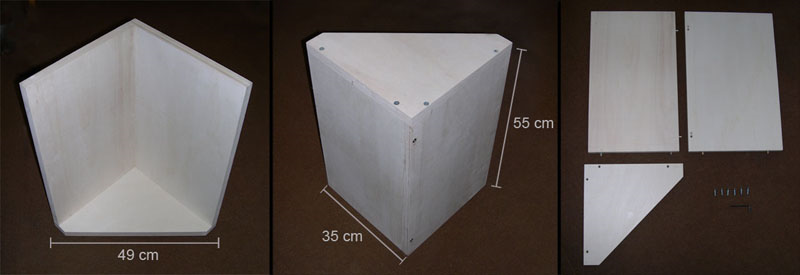
\includegraphics[width=0.9\textwidth]{buildingThreeDCalibrationObject}
\caption{Building 3D Calibration Object \cite{threeDExample_2014}}
\label{buildingThreeDCalibrationObject}
\end{figure}%
%
\begin{figure}[!t]
\centering
\subfloat[Six Points to Calibrate]{
	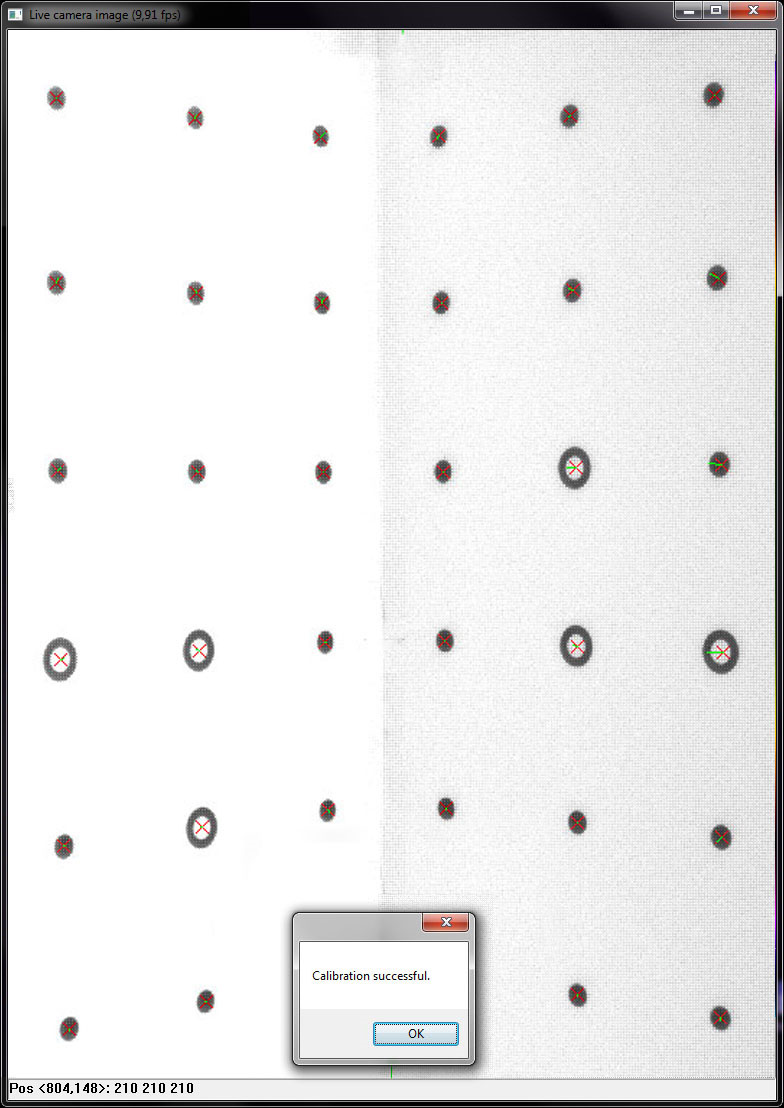
\includegraphics[height=0.6\textwidth, width=0.45\textwidth]{threeDSixPointsCalibrating}
	\label{threeDSixPointsCalibrating}
}
\subfloat[Reconstruction After Calibration]{
	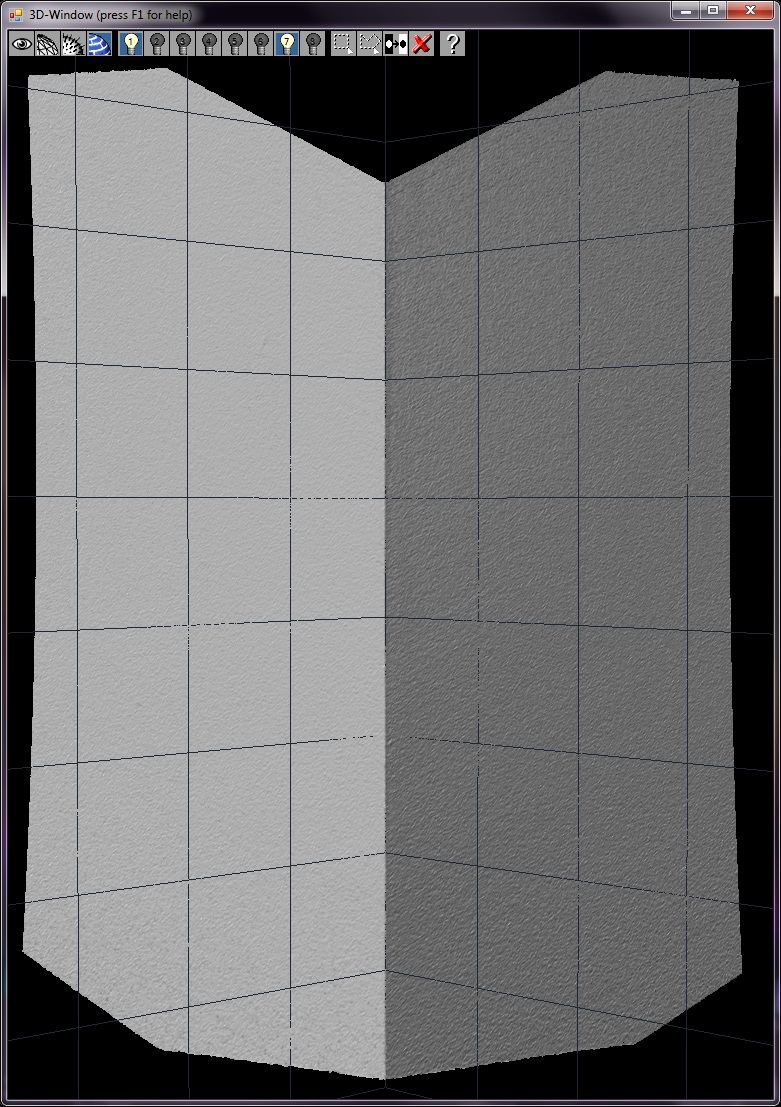
\includegraphics[height=0.6\textwidth, width=0.45\textwidth]{3DreconstructAfterCalibration}
	\label{3DreconstructAfterCalibration}
}
\caption{Three Dimension Object Camera Calibration \cite{threeDExample_2014}}
\label{twoPlanesCalibration}
\end{figure}%
%


%\begin{figure}[p]
%\centering
%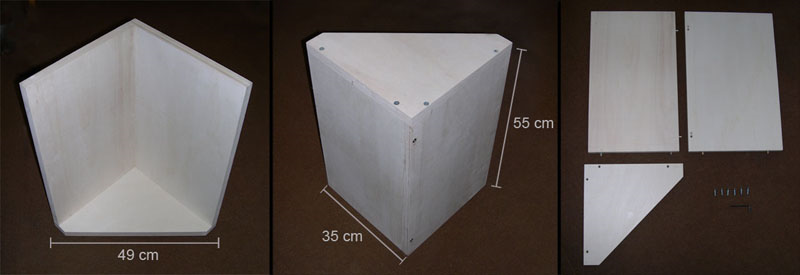
\includegraphics[width=0.8\textwidth]{buildingThreeDCalibrationObject}
%\caption{Building Three Dimension Object}
%\label{buildingThreeDCalibrationObject}
%\end{figure}%
%
%\begin{figure}[b]
%\centering
%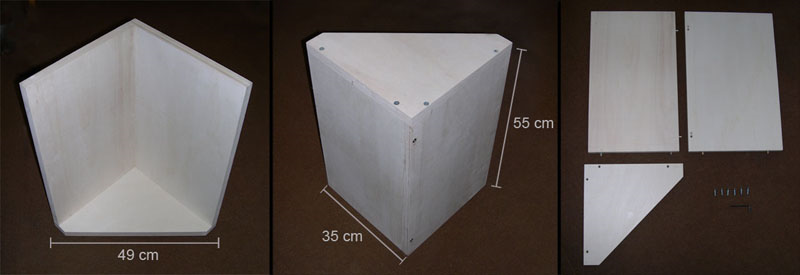
\includegraphics[width=0.8\textwidth]{buildingThreeDCalibrationObject}
%\caption{Building Three Dimension Object}
%\label{buildingThreeDCalibrationObject}
%\end{figure}%




%\\\\%

Zhengyou Zhang, a Chinese professor of computer science, IEEE and ACM Fellow and a specialist in computer vision and graphics, has deep studies on camera calibration from one-dimension calibration to tree-dimension calibration \cite{zhangCalibration1_2004} \cite{zhangCalibration2_2000} \cite{Zhengyou04}. The accuracy of calibration from 1D to 3D is getting better, but the calibration system setting-up needs more and more work and cost as well. One dimension object is suitable for calibrating multiple cameras at once. Two dimension planer pattern approaches seems to be a good compromise, with good accuracy and simple setup. Also using the three dimension method for calibration, Kai \cite{Kai10} derived the per-pixel  beam equation, the linear relationship that could map to \(X^w/Y^w\) from \(Z^w\) as eqn.~\ref{kaiBeamEquation} shows, directly from pinhole camera matrix \(M\) for every single pixel. That is to say, we could easily look up \(X^w/Y^w\) after calibration once found the way to get \(Z^w\).

\begin{equation}
\begin{aligned}
X^w_{[row, \, col]} = c_{[row, col]}Z^w_{[row, \, col]}+d_{[row, col]}
\\%
Y^w_{[row, \, col]} = e_{[row, col]}Z^w_{[row, \, col]}+f_{[row, col]}
\end{aligned}
\label{kaiBeamEquation}
\end{equation}%
\noindent
where \(c/d/e/f\) are per-pixel coefficients for the linear beam equations, and the subscripts [\(row, \, col\)] are corresponding per-pixel image coordinates.

%D[r, c] ~= Z^w[r, c] -- > (X^c, Y^c)
%Z^w[r, c] = Z^c[r, c] = D[r,c]

%%%%%%%%%%%%%%%%%%%%%%%%%%%%%%%%%%%%%%%%%%%%%%%%%%%%%
%%%%%%%%%%                                                                                                   %%%%%%%%%%
%%%%%%%%%%      4.        Lens Distortion Removal                                                %%%%%%%%%%%
%%%%%%%%%%                                                                                                    %%%%%%%%%%%
%%%%%%%%%%%%%%%%%%%%%%%%%%%%%%%%%%%%%%%%%%%%%%%%%%%%%%

\section{Lens Distortion}
%* distortion equation
%
\begin{figure}[b]
\centering
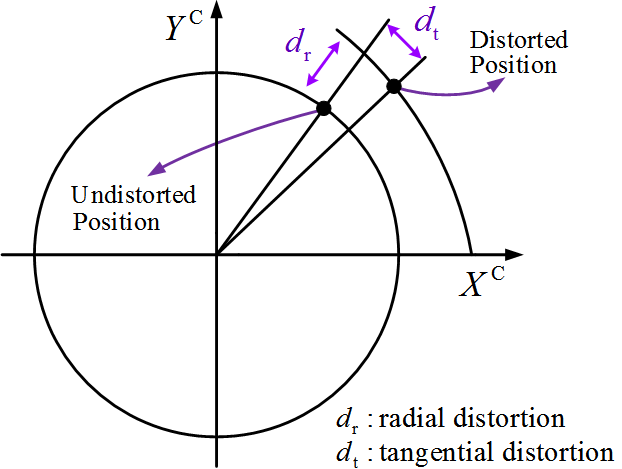
\includegraphics[width=0.65\textwidth]{RadialAndTangentialDistortion}
\caption{Radial and Tangential Distortion Affection In Image Space}
\label{RadialAndTangentialDistortion}
\end{figure}%
\indent
All above in Chapter \ref{chapterTraditionalCalibration} are talking about the ideal pinhole camera, without lenses. Whereas in practical, as a result of several types of imperfections in the design and assembly of lenses composing the camera optical system, there are always lens distortions for a camera and the expressions in eqn.~\ref{twoDRelativeFromCamToIm} are not valid any more. Lens distortion could be classified into two groups \cite{distortion1_1992} : radial distortion, and tangential distortion. Imperfect lens shape causes light rays bending more near the edges of a lens than they do at its optical center. The smaller the lens, the greater the distortion. Barrel distortions happen commonly on wide angle lenses, where the field of view of the lens is much wider than the size of the image sensor. Improper lens assembly will lead to tangential distortion, which occurs when the lens and the image plane are not parallel. fig.~\ref{RadialAndTangentialDistortion} shows how radial distortion \(d_\text{r}\) and tangential distortion \(d_\text{t}\) affect the object point position in the image. Note that both of radial distortion and tangential distortion are with respect to image space row and column, and what we will take later is negative distortion instead of positive. Distortions are present because the field of view (FoV) in camera space has been affected by the lens. For most consumer RGB-D cameras with cheap lens, their distortions are usually barrel distortions (negative distortion) resulted by the enlarged field  of view in the camera space, because the larger view was squeezed into the sensor. Fig.~\ref{DistortionComprehension} intuitively shows how the lens enlarged the field of view of in the camera space and then generates the barrel distortions.
%
\begin{figure}[t]
\centering
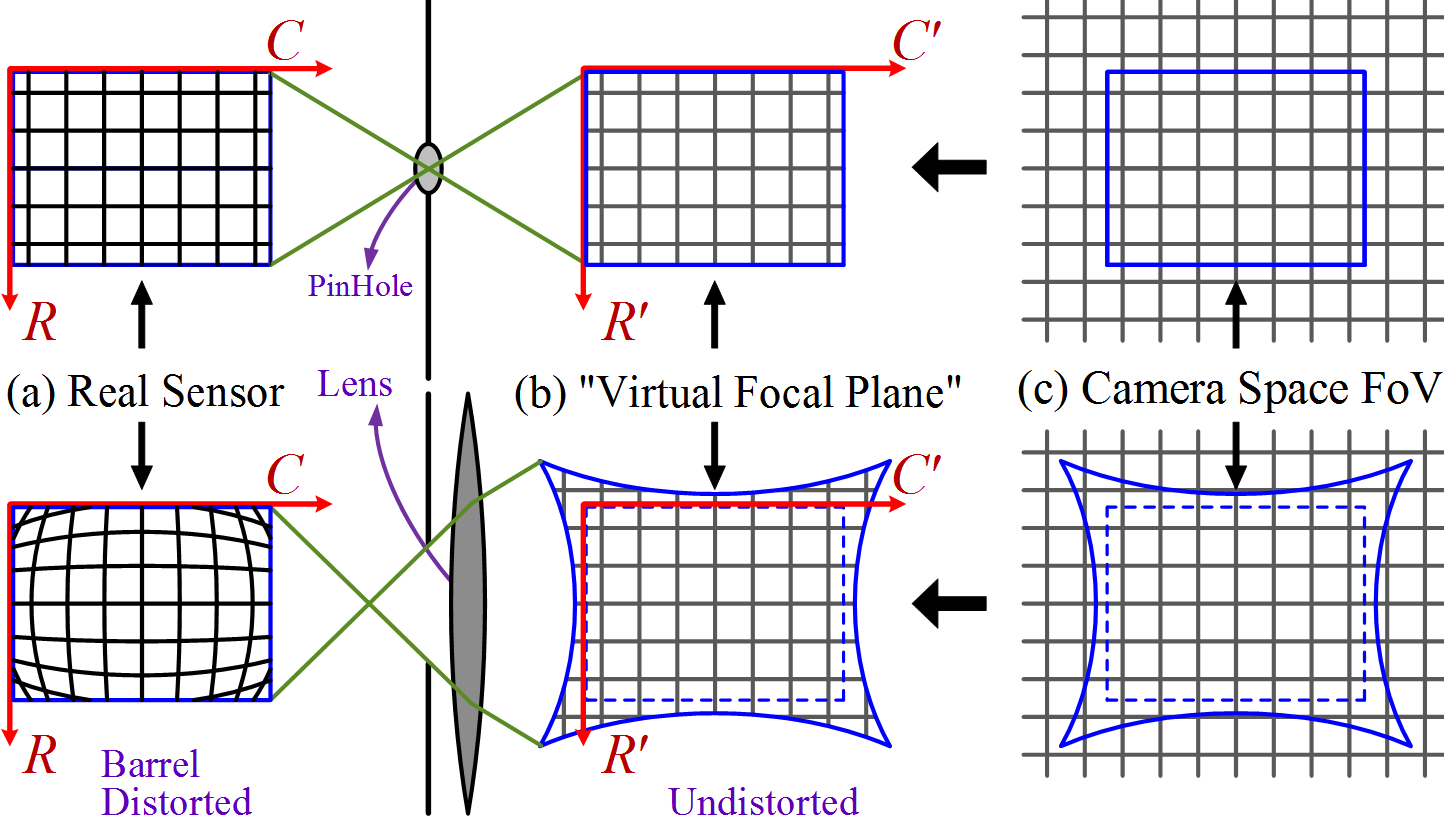
\includegraphics[width=\textwidth]{DistortionComprehension}
\caption{From Camera Space to Image Space with Lens Distortions}
\label{DistortionComprehension}
\end{figure}%

There are (a)(b)(c) three parts shown in fig.~\ref{DistortionComprehension}. Each part has the pinhole camera only on the top, in contrast to the camera-with-lens situation at the bottom. To understand how the barrel distortion happens, we should go through from part (c) to part (a). In part (c), the gray background uniform grid is the \enquote{object} our that the camera is going to observe, and the blue frames shows the FoV of the camera in the camera space. Due to the fact that, there will be worse and worse distortions as one pixel goes from the center to the edge, the enlarged FoV of a camera with lens in the camera space is in pincushion (or star) shape. With the enlarged Fov is mapped to the \enquote{Virtual Focal Plane}, as defined in fig.~\ref{PinHoleVirtualFocalPlane}, the pincushion shape doesn't change because rays from the camera space have not gone through the lens yet. Note that we quoted the \enquote{Virtual Focal Plane} because the image on this virtual plane, when considering lens distortion, does not equal to the real focal plane (where the sensor is) any more. We can tell from part (b) that, even though the image space coordinates still are composed of \(Col\) and \(Row\), their ranges have changed from positive integers only to the whole real integers that include negative ones. But the sensor never changes, and so the image space in part (a) still has its range of positive integers. With rays going through the lens, the pincushion-shape FoV (the frame in blue) will be squeezed into a small rectangle, and thus we get the image in the real focal plane with its background grid showing a barrel distorted shape.%
\\\indent%
With lens distortions counted, eqn.~\ref{twoDRelativeFromCamToIm} now needs to be changed into 
%
\begin{equation}
\left[ \begin{array}{c} \text{C'}_\text{r} \\ \text{R'}_\text{r} \end{array} \right] %
= f %
\left[ \begin{array}{c} \text{X}_\text{C}/\text{Z}_\text{C} \\ \text{Y}_\text{C}/\text{Z}_\text{C} \end{array} \right]%
\label{undistortedRelativeFromCamToIm}
\end{equation}
where \(\text{C'}_\text{r}\) and \(\text{R'}_\text{r}\) denote the relative pixel distance on the undistorted \enquote{Virtual Focal Plane}, whose FoV is pincushion-shape and image coordinates' ranges include negative integers.%
\\\indent%
Duane \cite{distortion2_1966} gave the lens distortion equation, and the undistorted \(Col\) and \(Row\) (\(C'/R'\) in our notation) can be expressed as power series in radial distance \(r = \sqrt{C^2 + R^2}\):
%
\begin{equation}
\begin{aligned}
C' =  C (1 + k_1 r^2 + k_2 r^4 + k_3 r^6) + [p_1 (r^2 + 2 C^2) + 2 p_2 CR] %
\\
R' =  R (1 + k_1 r^2 + k_2 r^4 + k_3 r^6) + [p_2 (r^2 + 2 R^2) + 2 p_1 CR]
\end{aligned}
\label{lensDistortion}
\end{equation}%
%
\noindent
where higher order parameters are omitted for being negligible; \((C', \, R')\) denote the undistorted pixels in the \enquote{Virtual Focal Plane}, \((C, \, R)\) denote the distorted pixel in real sensor image, \(k_i\)'s are coefficients of radial distortion, and \(p_j\)'s are coefficients of tangential distortion. The five parameters \(k_1/k_2/k_3/p_1/p_2\) are usually called distortion parameters. With the distortion parameters calculated, the distorted \((C, \, R)\) could be undistorted into \((C', \, R')\), and then \((C', \, R')\) could be used to generate the world space \(X^w/Y^w/Z^w\) with intrinsic and extrinsic parameters.
%

%%%%%%%%%%%%%%%%%%%%%%%%%%%%%%%%%%%%%%%%%%%%%%%%%%%%%
%%%%%%%%%%                                                                                                   %%%%%%%%%%
%%%%%%%%%%      4.       Summation                                                                  %%%%%%%%%%%
%%%%%%%%%%                                                                                                    %%%%%%%%%%%
%%%%%%%%%%%%%%%%%%%%%%%%%%%%%%%%%%%%%%%%%%%%%%%%%%%%%%

\section{Summation}
%
\indent
\indent In this chapter, a pinhole camera model is introduced in detail, which is expressed as a 3x4 matrix \(M\) that could help map from the world space 3D coordinate to image space 2D coordinates. The 3x4 matrix \(M\) can be decomposed into two separate matrix, the intrinsic matrix \(K\) and extrinsic matrix \([R_{3*3}\,\,T_{3*1}]\), each of them corresponds to one of the two parts of the pinhole camera model. The extrinsic matrix \([R_{3*3}\,\,T_{3*1}]\) consists of parameters outside the camera, which help map from 3D world space to 3D camera space. While the intrinsic matrix \(K\) consists of parameters all from the camera itself, which help map from the 3D camera space to 2D image space. After the pinhole camera model, various camera calibration techniques are discussed, all of which are based on the determination of the pinhole camera matrix \(M\) and then the recovery of the intrinsic matrix \(K\) and extrinsic matrix \([R_{3*3}\,\,T_{3*1}]\). Considering the lens distortions in practical, a lens distortions correction model (with  \(k_1/k_2/k_3/p_1/p_2\) five parameters) is given to undistort the lens distortions. 
%
\begin{figure}[t]
\centering
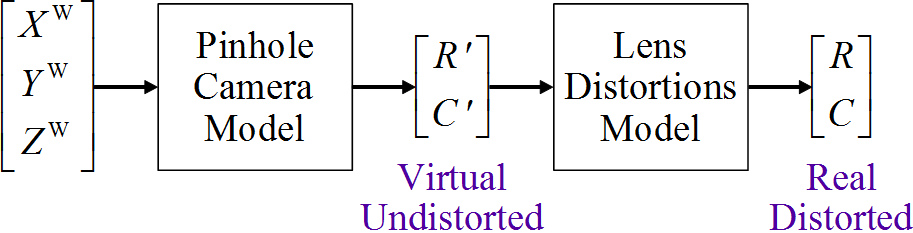
\includegraphics[width=0.6\textwidth]{flowChart}
\caption{Traditional Camera Calibration Flow Char}
\label{flowChart}
\end{figure}%
\\\indent
Fig.~\ref{flowChart} shows the flow chart of the whole traditional camera calibration method based on the pinhole camera model. Considering the lens distortions, both of the pinhole camera model (matrix \(M\)) and the lens distortions model (five parameters for undistortion) need to be determined. The pinhole camera model can help map from the world space (\(X^\text{W}, \, Y^\text{W}, \, Z^\text{W}\)) to the undistorted image space (\(R', \, C'\)), which are on the \enquote{Virtual Focal Plane} as noted in fig.~\ref{DistortionComprehension}. And the lens distortion model help remove the lens distortions by mapping from (\(R', \, C'\)) to (\(R, \, C\)). The pinhole camera model can be determined by eqn.~\ref{determinationOfPinhole3x4}, and the lens distortion model could be determined by eqn.~\ref{lensDistortion}.



























%Pinhole camera model is wildly used in 3D camera's reconstruction, however, it is not able to handle non-linear radial distortion. In this chapter, a pinhole model based 3D camera calibration method (derived from a 3D reconstruction example of structured light method) will be discussed in detail, and then extended into two newly proposed calibration methods.
%
%%%%%%%%%%%%%%%%%%%%%%%%%%%%%%%%%%%%%%%%%%%%%%%%%%%%%%
%%%%%%%%%%%                                                     %%%%%%%%%%%%%%%%%%%%%%%%%%
%%%%%%%%%%% 2.1   Pinhole Camera Model                   %%%%%%%%%%%%%%%%%%%%%%%%
%%%%%%%%%%%                                                     %%%%%%%%%%%%%%%%%%%%%%%%
%%%%%%%%%%%%%%%%%%%%%%%%%%%%%%%%%%%%%%%%%%%%%%%%%%%%%%%
%
%\section{Pinhole Camera Model}
%\label{sectionPinholeCamera}
%%%
%fig.~\ref{PinholeCameraModel} shows the basic diagram of a pinhole camera model \cite{Maria10} \cite{Zhengyou04} with a reflected image plane for friendly intuition. From this model, the mapping between 3D space world coordinate and the image plane row and column could be separated into two parts of transformations. The first part is the transformation between world coordinates system \(X\)/\(Y\)/\(Z\) and camera coordinate system \(U\)/\(V\)/\(W\) , which forms a 4x4 perspective transformation matrix (\textbf{extrinsic calibration}) that works for 3D rotation and translation. And the second part is the mapping between 3D camera coordinates system \(U\)/\(V\)/\(W\) and 2D image plane coordinates \(u\)/\(v\), which forms a 3x3 perspective transformation matrix (\textbf{intrinsic calibration}) that works for not only the rescaling between camera coordinates and virtual ideal image coordinates, but also for translating and skewing between the virtual ideal image plane and real image plane. %
%%
%\begin{figure}[h]
%\centering
%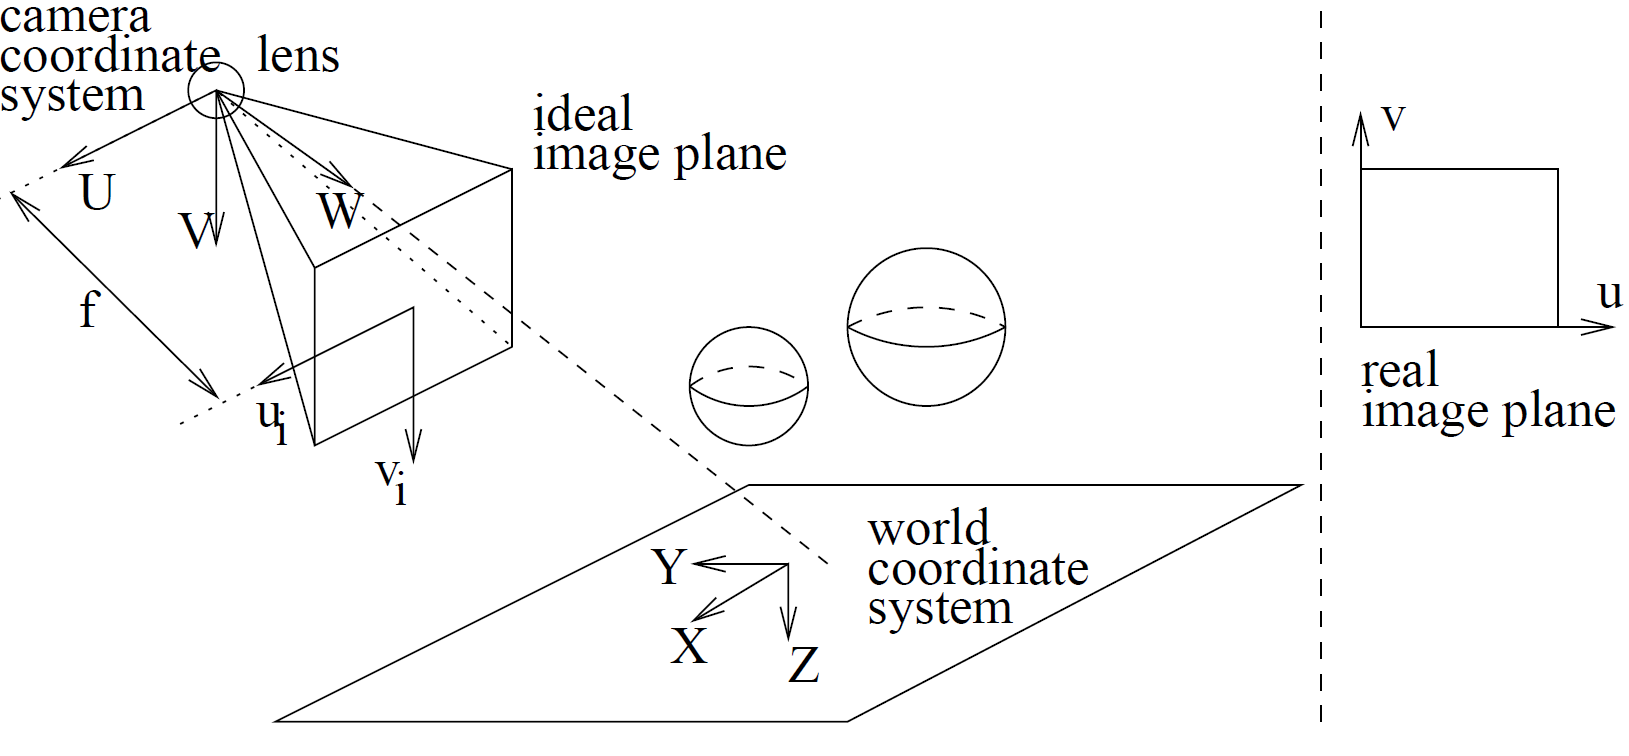
\includegraphics[width=\textwidth]{PinholeCameraModel}
%\caption{The pinhole camera model}
%\label{PinholeCameraModel}
%\end{figure}%
%%
%\\\par%
%\textbf{Extrinsic Calibration}\\
%Without any camera parameters, the extrinsic calibration formula could be written, through homogeneous coordinates, as
%%
%\begin{equation}
%\left[ \begin{array}{c} U \\ V \\ W \\ 1 \end{array} \right] %
%= %
%\begin{bmatrix} R & T \\ 0 & 1 \end{bmatrix} \times \left[ \begin{array}{c} X^w \\ Y^w \\ Z^w \\ 1 \end{array} \right]
%\end{equation}%
%%
%or for simplicity,
%\begin{equation}
%%
%\left[ \begin{array}{c} U \\ V \\ W \end{array} \right] %
%= %
%\begin{bmatrix} R & T \end{bmatrix} \cdot \left[ \begin{array}{c} X^w \\ Y^w \\ Z^w \end{array} \right]
%\label{extrinsicTransform}
%%
%\end{equation}%
%%
%where \((U, V, W)^T\) are the camera coordinates, and the transformation matrix component \([R\)  \(T]\), which is part of the 4x4 perspective matrix, is modeling rotation and translation , written as
%
%\begin{equation}
%%
%\left[ \begin{array}{cc} R & T \end{array} \right] %
%= %
%\begin{bmatrix}
% r_{11} & r_{12} & r_{13} & t_1 \\
% r_{21} & r_{22} & r_{23} & t_2 \\
% r_{31} & r_{32} & r_{33} & t_3
%\end{bmatrix}
%%
%\end{equation}
%\\\par
%%
%%
%\textbf{Intrinsic Calibration}\\
%Intrinsic Calibration could be separated into two sections. The first section is to rescale from camera coordinates to virtual ideal image coordinates. For a easier integration of two sections, the first section's formula is given through both of 2D coordinates to homogeneous coordinates.\par
%%
%\quad\quad2D coordinates:%
%\begin{equation}
%%
%W \left[ \begin{array}{c} u^i \\ v^i  \end{array} \right] %
%= f %
%\left[ \begin{array}{c} U \\ V \end{array} \right]%
%%
%\end{equation}
%
%\quad\quad Homogeneous coordinates:\par
%\begin{equation}
%%
%W \left[ \begin{array}{c} u^i \\ v^i \\ 1 \end{array} \right] %
%= %
%\left[ \begin{array}{c} fU \\ fV \\ W \end{array} \right]%
%=  \begin{bmatrix} f & 0 & 0 \\ 0 & f & 0 \\ 0 & 0 & 1 \end{bmatrix} \cdot %
%\left[ \begin{array}{c} U \\ V \\ W \end{array} \right]%
%\label{section_1}
%\end{equation}%
%\\\par
%%
%The second section is for translating and skewing between the virtual ideal image plane \(u^i\)/\(v^i\) and real image plane \(u^r\)/\(v^r\),  %
%
%\begin{equation}
%%
%\left[ \begin{array}{c} u^r \\ v^r \\ 1 \end{array} \right] %
%=  \begin{bmatrix} s_u & s_\theta & u_0 \\ 0 & s_v & v_0 \\ 0 & 0 & 1 \end{bmatrix} \cdot %
%\left[ \begin{array}{c} u^i \\ v^i \\ 1 \end{array} \right]%
%\label{section_2}
%\end{equation}%
%where \((u_0, v_0)\) denotes the optical center (or principal point), \([s_u, s_v]\) are skew coefficients in pixels along \(u\) and  \(v\) axes , and  \(s_\theta\) is an skewed angle generated by \(s_u\) and  \(s_v\). To combine eqn.~\ref{section_1} and eqn.~\ref{section_2}, we could get %
%
%\begin{equation}
%%
%W \left[ \begin{array}{c} u^r \\ v^r \\ 1 \end{array} \right] %
%=  \begin{bmatrix} s_u & s_\theta & u_0 \\ 0 & s_v & v_0 \\ 0 & 0 & 1 \end{bmatrix} \cdot%
% \begin{bmatrix} f & 0 & 0 \\ 0 & f & 0 \\ 0 & 0 & 1 \end{bmatrix} \cdot %
%\left[ \begin{array}{c} U \\ V \\ W \end{array} \right]%
%=  \begin{bmatrix} f_u & s & u_0 \\ 0 & f_v & v_0 \\ 0 & 0 & 1 \end{bmatrix} \cdot%
%\left[ \begin{array}{c} U \\ V \\ W \end{array} \right]%
%%
%\label{intrinsicTransform}
%\end{equation}%
%%
%where \([f_u,\, f_v]\) denote focal lengths in pixels along \(u\) and \(v\) after skewing, and \(s\) is a new skew coefficient after combination.\\\par%
%%
%\textbf{Generic Perspective Matrix of the Pinhole Camera Model}\par%
%
%After both of the extrinsic and intrinsic transformation matrices have been derived, the generalization formula of the pinhole camera model could be derived, combining eqn.~\ref{extrinsicTransform} and \ref{intrinsicTransform}, as
%
%\begin{equation}
%%
%k \left[ \begin{array}{c} u^r \\ v^r \\ 1 \end{array} \right] %
%=  \begin{bmatrix} f_u & s & u_0 \\ 0 & f_v & v_0 \\ 0 & 0 & 1 \end{bmatrix} \cdot%
%\begin{bmatrix} R & T \end{bmatrix} \cdot \left[ \begin{array}{c} X^w \\ Y^w \\ Z^w \\ 1 \end{array} \right]%
%=  C \cdot \left[ \begin{array}{c} X^w \\ Y^w \\ Z^w \\ 1 \end{array} \right]%
%%
%\label{detailedPerspectivePinholeCameraMatrix}
%\end{equation}%
%%
%where \(W\) on the left side has been replaced by \(k\) to be a more general proportion coefficient, and a combined matrix can be expressed as
%\begin{equation}
%%
%C %
%=  \begin{bmatrix} f_u & s & u_0 \\ 0 & f_v & v_0 \\ 0 & 0 & 1 \end{bmatrix} \cdot%
%\begin{bmatrix} R & T \end{bmatrix}%
%= \begin{bmatrix} 
%m_{11} & m_{12} & m_{13} & m_{14} \\
%m_{21} & m_{22} & m_{23} & m_{24} \\
%m_{31} & m_{32} & m_{33} & m_{34} \\
%\end{bmatrix}%
%%
%\label{genericPerspectivePinholeMatrix}
%\end{equation}%
%%
%The final 3x4 matrix C is considered as the generic perspective transformation matrix of a pinhole camera model, which gives a mapping between the 3D world coordinates and 2D real image coordinates. To inspect the pinhole camera matrix, its effects focuses on the taking care of linear processes of rotation, translation and skewing, given a perspective view. In other words, this 3x4 transformation matrix is specially for the removal perspective distortion . It is based on the homogeneous coordinates, while also limited by the linear system. And a mapping using this 3x4 transformation matrix between two coordinates can only be linear.
%\\\\%
%The pinhole camera matrix can be solved using least squares fit with known 3D points (\(X^w\), \(Y^w\), \(Z^w\)) and their corresponding image points (\(u^r\), \(v^r\)). With one point, based on eqn.~\ref{detailedPerspectivePinholeCameraMatrix} and \ref{genericPerspectivePinholeMatrix}, we can get
%\begin{equation}
%\begin{aligned}
%m_{11}X^w + m_{12}Y^w + m_{13}Z^w + m_{14} - m_{31}u^rX^w - m_{32}u^rY^w - m_{33}u^rZ^w - m_{34}u^r = 0%
%\\%
%m_{21}X^w + m_{22}Y^w + m_{23}Z^w + m_{24} - m_{31}v^rX^w - m_{32}v^rY^w - m_{33}v^rZ^w - m_{34}v^r = 0
%\end{aligned}
%\label{onePointEquationCR}
%\end{equation}%
%There are two equations for one point, and totally 12 unknowns to solve. We need at least six points to solve the 3x4 pinhole camera matrix. Using n-points least squares to solve the best fit, we can build a 2n equations matrix
%
%\begin{equation}
%\hspace*{-1cm}
%\begin{bmatrix} 
%X^w_1 & Y^w_1 & Z^w_1 & 1 & 0 & 0 & 0 & 0 & -u^r_1X^w_1 & -u^r_1Y^w_1 & -u^r_1Z^w_1 & -u^r_1\\
%0 & 0 & 0 & 0 & X^w_1 & Y^w_1 & Z^w_1 & 1 &  -v^r_1X^w_1 & -v^r_1Y^w_1 & -v^r_1Z^w_1 & -v^r_1\\
%X^w_2 & Y^w_2 & Z^w_2 & 1 & 0 & 0 & 0 & 0 & -u^r_2X^w_2 & -u^r_2Y^w_2 & -u^r_2Z^w_2 & -u^r_2\\
%0 & 0 & 0 & 0 & X^w_2 & Y^w_2 & Z^w_2 & 1 &  -v^r_2X^w_2 & -v^r_2Y^w_2 & -v^r_2Z^w_2 & -v^r_2\\
% & & & & & & & \vdots & & & & \\
%X^w_n & Y^w_n & Z^n_2 & 1 & 0 & 0 & 0 & 0 & -u^r_nX^w_n & -u^r_nY^w_n & -u^r_nZ^w_n & -u^r_n\\
%0 & 0 & 0 & 0 & X^w_n & Y^w_n & Z^w_n & 1 & -v^r_nX^w_n & -v^r_nY^w_n & -v^r_nZ^w_n & -v^r_n
%\end{bmatrix}
%\begin{bmatrix} 
%m_{11} \\ m_{12} \\ m_{13} \\ m_{14} \\
%m_{21} \\ m_{22} \\ m_{23} \\ m_{24} \\
%m_{31} \\ m_{32} \\ m_{33} \\ m_{34} 
%\end{bmatrix}
%=
%\begin{bmatrix} 
%0 \\ 0 \\ 0 \\ 0 \\
%\vdots \\ 0 \\ 0
%\end{bmatrix}
%\label{nPoints2nEquationCR}
%\end{equation}%
%
%
%Considering that this matrix is build on homogeneous system, there is no unique solution. There can always be a total-zeros solution. To make the solution unique, we select \(m_{34} = 1\), so that the homogeneous eqn.~\ref{nPoints2nEquationCR} could be changed into an inhomogeneous format like \(AX = B\), as eqn.~\ref{inHomogenousNPoints2nEquationCR} below.
%
%\begin{equation}
%\hspace*{-0.1cm}
%\begin{bmatrix} 
%X^w_1 & Y^w_1 & Z^w_1 & 1 & 0 & 0 & 0 & 0 & -u^r_1X^w_1 & -u^r_1Y^w_1 & -u^r_1Z^w_1\\
%0 & 0 & 0 & 0 & X^w_1 & Y^w_1 & Z^w_1 & 1 &  -v^r_1X^w_1 & -v^r_1Y^w_1 & -v^r_1Z^w_1\\
%X^w_2 & Y^w_2 & Z^w_2 & 1 & 0 & 0 & 0 & 0 & -u^r_2X^w_2 & -u^r_2Y^w_2 & -u^r_2Z^w_2\\
%0 & 0 & 0 & 0 & X^w_2 & Y^w_2 & Z^w_2 & 1 &  -v^r_2X^w_2 & -v^r_2Y^w_2 & -v^r_2Z^w_2\\
% & & & & & & & \vdots & & &\\
%X^w_n & Y^w_n & Z^n_2 & 1 & 0 & 0 & 0 & 0 & -u^r_nX^w_n & -u^r_nY^w_n & -u^r_nZ^w_n\\
%0 & 0 & 0 & 0 & X^w_n & Y^w_n & Z^w_n & 1 & -v^r_nX^w_n & -v^r_nY^w_n & -v^r_nZ^w_n
%\end{bmatrix}
%\begin{bmatrix} 
%m_{11} \\ m_{12} \\ m_{13} \\ m_{14} \\
%m_{21} \\ m_{22} \\ m_{23} \\ m_{24} \\
%m_{31} \\ m_{32} \\ m_{33}
%\end{bmatrix}
%=
%\begin{bmatrix} 
%u^r_1 \\ v^r_1 \\ u^r_2 \\ v^r_2 \\
%\vdots \\ u^r_n \\ v^r_n
%\end{bmatrix}
%\label{inHomogenousNPoints2nEquationCR}
%\end{equation}%
%
%Using pseudo inverse, eqn.~\ref{inHomogenousNPoints2nEquationCR} can be solved by \(X = (A^TA)^{-1}A^TB\), where \(X\) is an 11-elements vector and \(X(1)\)  \texttildelow \, \(X(11)\) correspond to \(m_{11}\) \texttildelow \, \(m_{33}\). And the 3x4 pinhole camera matrix, eqn.~\ref{genericPerspectivePinholeMatrix}, will be determined as
%
%\begin{equation}
%C =
%\begin{bmatrix} 
%X(1) & X(2) & X(3) & X(4) \\
%X(5) & X(6) & X(7) & X(8) \\
%X(9) & X(10) & X(11) & 1
%\end{bmatrix}
%\label{determinationOfPinhole3x4}
%\end{equation}%
%

%%%%%%%%%%%%%%%%%%%%%%%%%%%%%%%%%%%%%%%%%%%%%%%%%%%%%%%
%%%%%%%%%%                                                                              %%%%%%%%%%%%%%%%%%%%%
%%%%%%%%%% 2.2   Structured Light 3D Reconstruction in Real-Time   %%%%%%%%%%%%%%%%%%%
%%%%%%%%%%                                                                                 %%%%%%%%%%%%%
%%%%%%%%%%%%%%%%%%%%%%%%%%%%%%%%%%%%%%%%%%%%%%%%%%%%%
%\section{Structured Light 3D Reconstruction in Real-Time}
%\label{sectionSL3DReconstructionRealTime}
%Using a 3D reconstruction method of structured light, applying Phase Measuring Profilometry (PMP) technique, a per-pixel 3D camera calibration method based on pinhole camera model is detailedly introduced in this section. Both of the advantage and disadvantage are discussed.
%%
%%
%\begin{figure}[H]
%\centering
%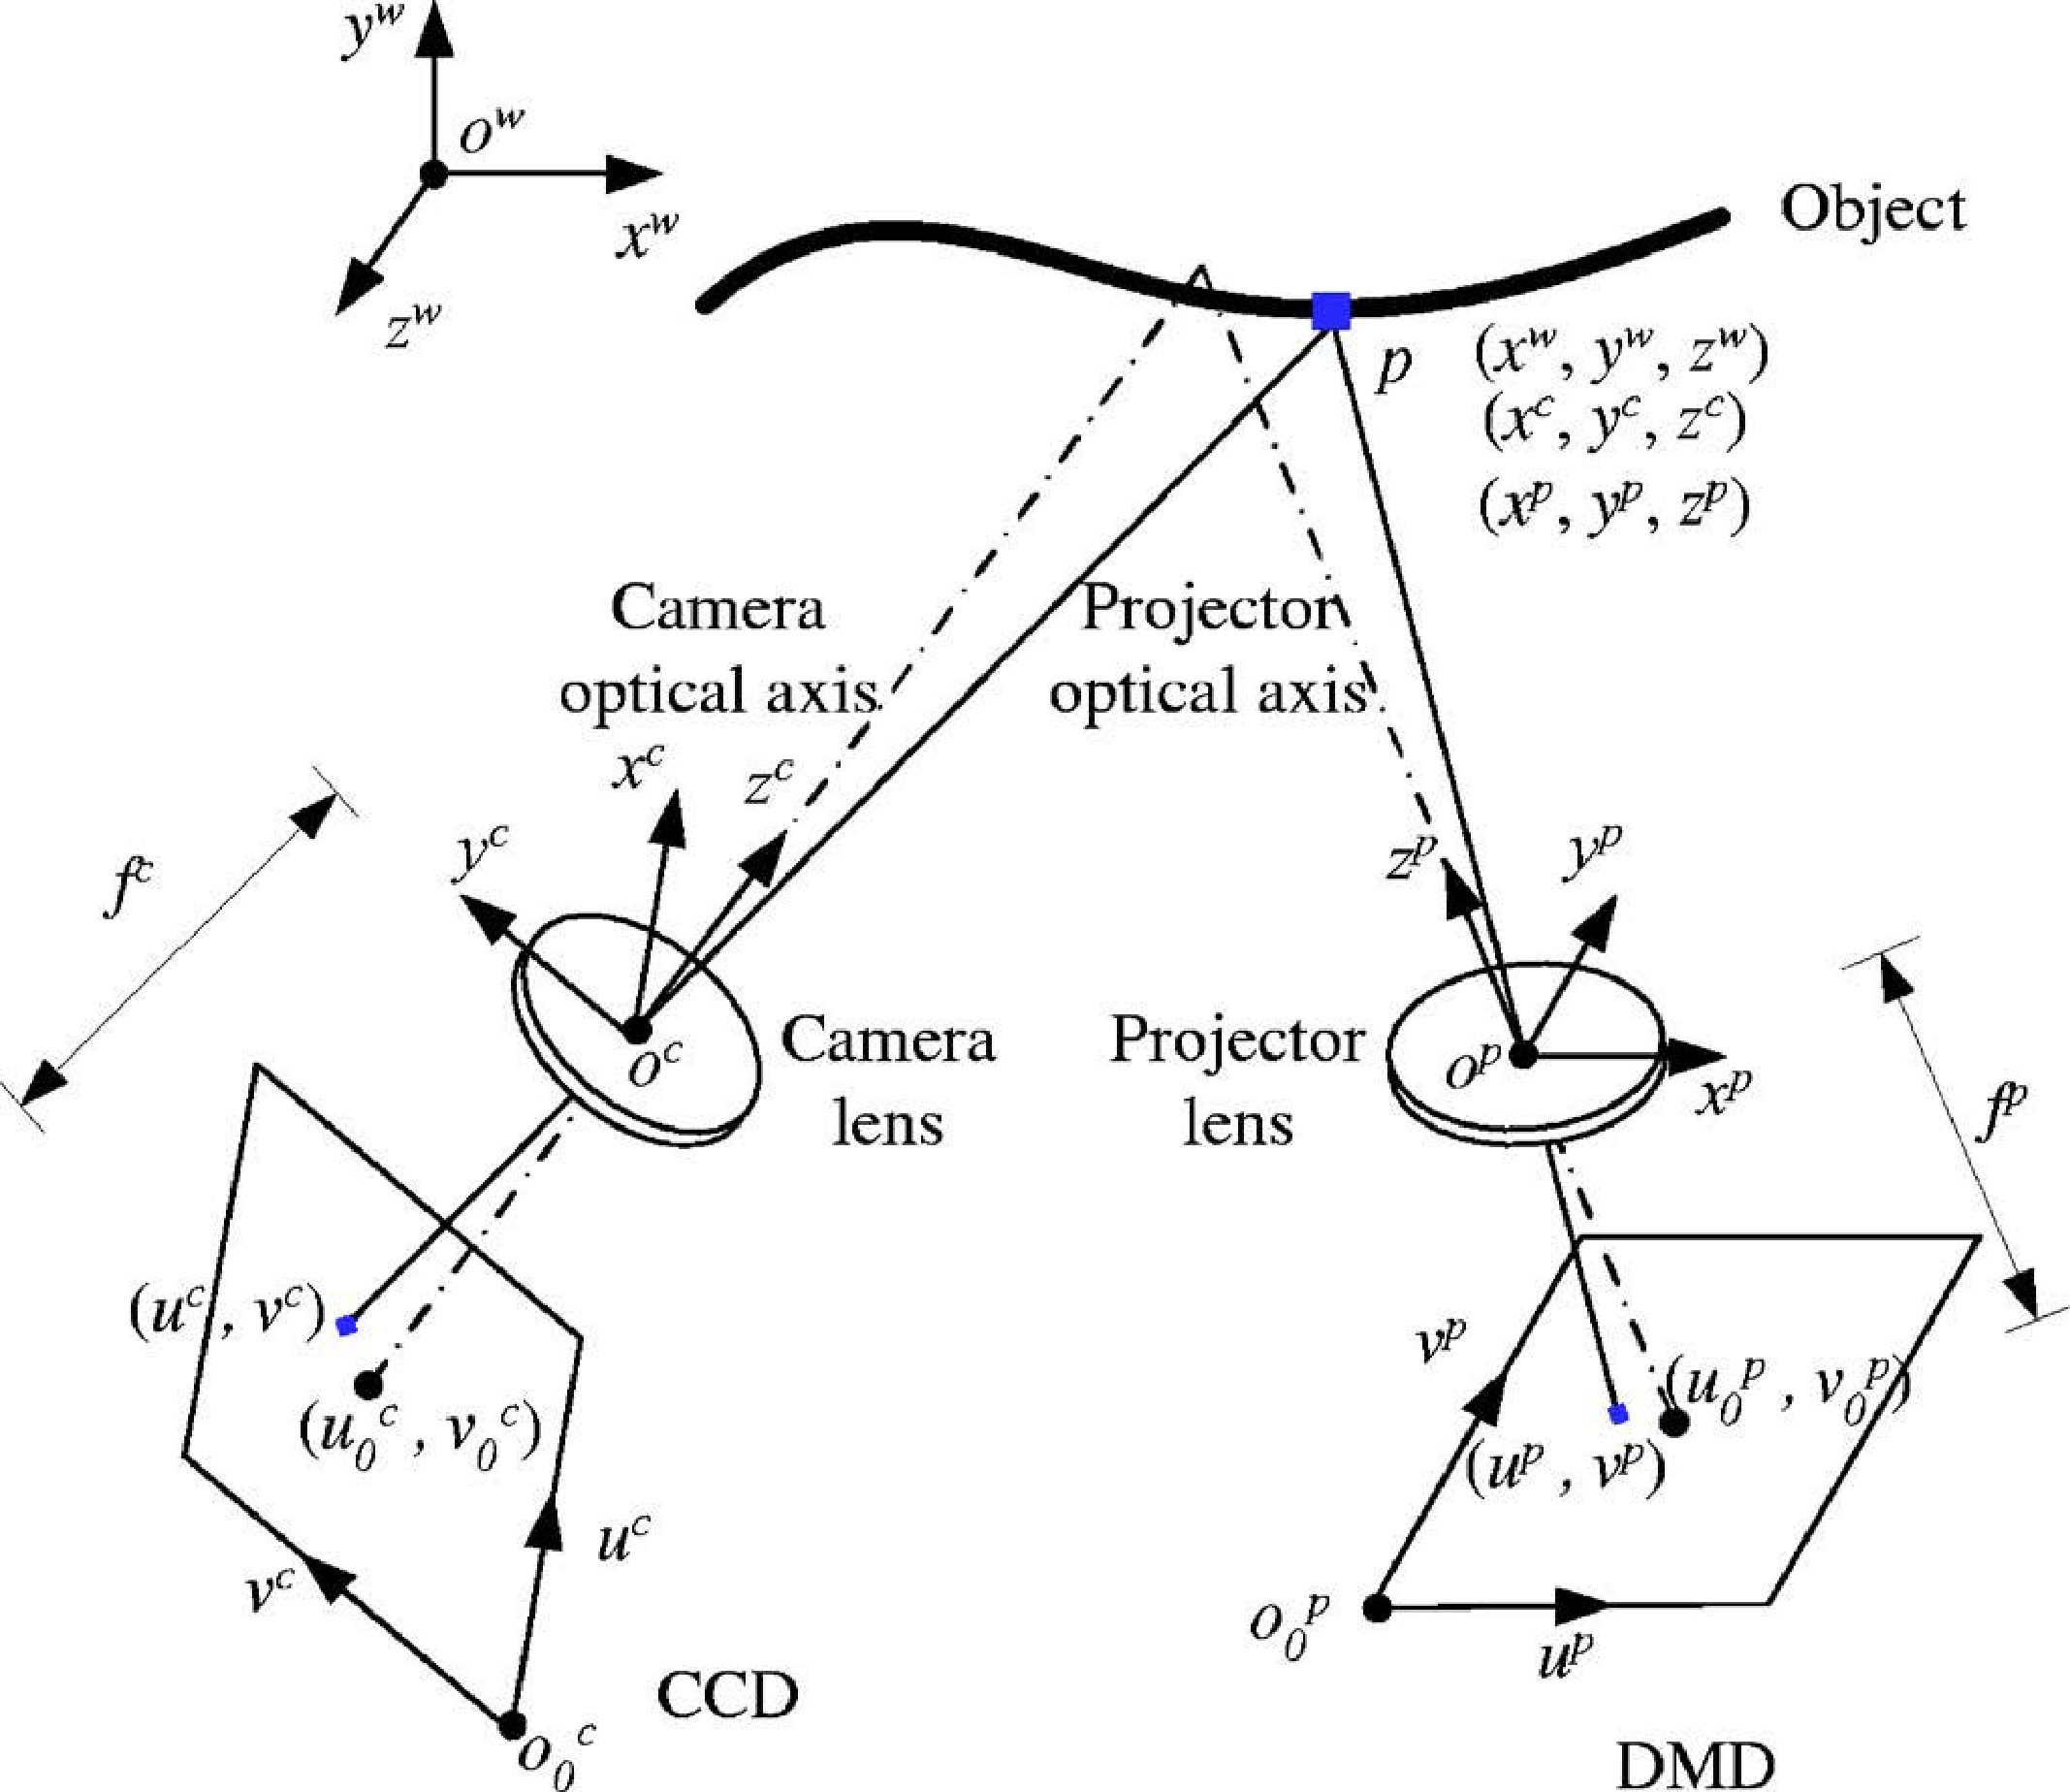
\includegraphics[width=0.7\textwidth]{SLPMPConfiguration}
%\caption{SL PMP Configuration Diagram \cite{Song06}}
%\label{SLPMPConfiguration}
%\end{figure}%
%%
%A 3D shape measurement system consists of a Charge-Coupled Device (CCD) camera and a Digital Micro-mirror Device (DMD) projector. 2D image pattern strategies are always preferred for fast scanning if a DMD projector is involved
%[**]%J. Salvi, J. Pages, and J. Batlle, \Pattern codication strategies in structured light systems," Pattern Recognition 37, 827{849 (2004).
% \cite{Song06}.
%And the multi-shot pattern Phase Measuring Profilometry strategy was used for its properties of robust and accuracy.
%With PMP information encoded in the structured light pattern projected onto the target, the CCD camera could capture a series of images that contains PMP informatio. Triangulation analyzing could be used to extract the 3D world coordinates for each points of the target profile, by a determination of the relationships among CCD camera, DMD projector, and the target object. A system configuration of PMP application is given in fig.~\ref{SLPMPConfiguration}.%
%\\\\%
%PMP method uses either vertical or horizontal sinusoid patterns, which could be described as:
%
% \begin{equation}
%%
%I^p_n(x^p, \, y^p) %
%= A^p(x^p, \, y^p) + B^p(x^p, \, y^p)Cos(2\pi fy^p - \frac{2\pi n}{N})
%%
%\end{equation}%
%%
%where \((x^p, \, y^p)\) denotes the coordinates of every single pixel in the projector, \(I^p_n\) denotes the intensity of the corresponding pixels, \(A^p\) and \(B^p\) are constants, \(f\) is the frequency of sine wave. The subscript \(n\) represents the index of phase shift, while capital \(N\) is the total number of phase shift.\par%
%%
%%
% \begin{figure}[h]
%%\centering
%\hspace*{-2cm} 
%\subfloat[Pattern 0][1]{
%
\includegraphics[width=0.3\textwidth]{Pattern0}
%\label{fig:subfig1}}
%\subfloat[Pattern 1][2]{
%
\includegraphics[width=0.3\textwidth]{Pattern1}
%\label{fig:subfig2}}
%\subfloat[Pattern 2][3]{
%
\includegraphics[width=0.3\textwidth]{Pattern2}
%\label{fig:subfig3}}
%%\qquad
%\subfloat[Pattern 3][4]{
%
\includegraphics[width=0.3\textwidth]{Pattern3}
%\label{fig:subfig4}}
%\caption{PMP base frequency patterns}
%\label{PMPFrequencyPatterns}
%\end{figure}%
%%
%%\begin{figure}
%%    \centering
%%    \hspace*{-3cm} 
%%    \begin{subfigure}[b]{0.3\textwidth}
%%            
\includegraphics[width=\textwidth]{Pattern0}
%%            \caption{Pattern 0}
%%    \end{subfigure}%
%%    ~ 
%%    \begin{subfigure}[b]{0.3\textwidth}
%%            
\includegraphics[width=\textwidth]{Pattern1}
%%            \caption{Pattern 1}
%%    \end{subfigure}
%%    ~ 
%%    \begin{subfigure}[b]{0.3\textwidth}
%%            
\includegraphics[width=\textwidth]{Pattern2}
%%            \caption{Pattern 2}
%%    \end{subfigure}
%%    ~ 
%%    \begin{subfigure}[b]{0.3\textwidth}
%%            
\includegraphics[width=\textwidth]{Pattern3}
%%            \caption{Pattern 3}
%%    \end{subfigure}
%%    \caption{PMP base frequency patterns}
%%    \label{PMPFrequencyPatterns}
%%\end{figure}
%%
%%
%%
%fig.~\ref{PMPFrequencyPatterns} shows a group of sine wave patterns, where the number of total phase shift \(N = 4\) and frequency \(f = 1\). From viewpoint of the camera, the sinusoid patterns is distorted by the target surface topology, so that the captured images could be expressed as 
%
% \begin{equation}
%%
%I^c_n(x^c, \, y^c) %
%= A^c(x^c, \, y^c) + B^c(x^c, \, y^c)Cos[\phi(x^c,\, y^c) - \frac{2\pi n}{N}]
%%
%\end{equation}%
%%
%where\((x^c, \, y^c)\) denotes the coordinates of every single pixel in the camera, and the term \(\phi(x^c,\, y^c)\) represents the corresponding phase value, which could be computed as follows [6]\par
% % Very High Resolution 3-D surface Scanning Using Multi-Frequency Phase Measuring Profilometry
% \begin{equation}
%%
%\phi(x^c,\, y^c) %
%= arctan\Bigg[\frac{\sum^N_{n=1}I(x^c,\,y^c)Sin(2\pi n / N)}{\sum^N_{n=1}I(x^c,\,y^c)Cos(2\pi n / N)} \Bigg]
%%
%\label{equationArctangent}
%\end{equation}
%%
%%
%After the camera term  \(\phi(x^c,\, y^c)\)  for every single pixel is computed, the corresponding projector coordinate \(y^p\) could be derived through equation\par
%
%\begin{equation}
%%
%y^p %
%= \phi(x^c,\, y^c) / (2\pi f)
%%
%\end{equation}%
%%
%With the knowledge of \(y^p\), the perspective information between camera and projector is the last step to go for applying triangulation analysis to extract world coordinates. Based on pinhole camera model, the perspective matrices for both of the CCD camera and DMD projector, as will be derived later in section \ref{sectionPinholeCamera} eqn.~\ref{genericPerspectivePinholeMatrix}, are written as [7]\par
%% J. Li, L. G. Hassebrook, and C. Guan, \Optimized two-frequency phasemeasuring-prolometry light-sensor temporal-noise sensitivity," Journal of the Optical Society of America A 20, 106{115 (2003).
%
%\begin{equation}
%%
%M^c %
%= \begin{bmatrix} 
%m^c_{11} & m^c_{12} & m^c_{13} & m^c_{14} \\
%m^c_{21} & m^c_{22} & m^c_{23} & m^c_{24} \\
%m^c_{31} & m^c_{32} & m^c_{33} & m^c_{34} \\
%\end{bmatrix}%
%%
%%\label{genericPerspectivePinholeMatrix}
%\end{equation}%
%%
%and 
%
%\begin{equation}
%%
%M^p %
%= \begin{bmatrix} 
%m^p_{11} & m^p_{12} & m^p_{13} & m^p_{14} \\
%m^p_{21} & m^p_{22} & m^p_{23} & m^p_{24} \\
%m^p_{31} & m^p_{32} & m^p_{33} & m^p_{34} \\
%\end{bmatrix}%
%%
%%\label{genericPerspectivePinholeMatrix}
%\end{equation}%
%%
%The mapping from 3D world coordinates to 2D camera coordinates are given by\par
%
%\begin{equation}
%%
%x^c %
%= \frac%
%{m^c_{11}X^w + m^c_{12}Y^w + m^c_{13}Z^w + m^c_{14}}%
%{m^c_{31}X^w + m^c_{32}Y^w + m^c_{33}Z^w + m^c_{34}}
%%
%\label{cameraXmapping}
%\end{equation}%
%%
%%
%\begin{equation}
%%
%y^c %
%= \frac%
%{m^c_{21}X^w + m^c_{22}Y^w + m^c_{23}Z^w + m^c_{24}}%
%{m^c_{31}X^w + m^c_{32}Y^w + m^c_{33}Z^w + m^c_{34}}
%%
%\label{cameraYmapping}
%\end{equation}%
%%
%%
%Likewise, the translation from 3D world coordinates to 2D projector coordinates are given by\par
%\begin{equation}
%%
%x^p %
%= \frac%
%{m^p_{11}X^w + m^p_{12}Y^w + m^p_{13}Z^w + m^p_{14}}%
%{m^p_{31}X^w + m^p_{32}Y^w + m^p_{33}Z^w + m^p_{34}}
%%
%\label{projectorXmapping}
%\end{equation}%
%%
%\begin{equation}
%%
%y^p %
%= \frac%
%{m^p_{21}X^w + m^p_{22}Y^w + m^p_{23}Z^w + m^p_{24}}%
%{m^p_{31}X^w + m^p_{32}Y^w + m^p_{33}Z^w + m^p_{34}}
%%
%\label{projectorYmapping}
%\end{equation}%
%%
%%
%Since three out of four equations \ref{cameraXmapping} \texttildelow \,\ref{projectorYmapping} are enough to solve \(X^{w}\),  \(Y^{w}\),  and \(Z^{w}\), and \(y^p\) is already calculated, the 3D world coordinates \(X^{w}\)/\(Y^{w}\)/\(Z^{w}\)  could be derived from Eqs  \ref{cameraXmapping},  \ref{cameraYmapping}, and \ref{projectorYmapping}\par%
%%
%\begin{equation}
%\hspace*{-0.3cm} 
%%
%\left[ \begin{array}{c} X^w\\ Y^w\\ Z^w\end{array} \right] %
%= %
%\begin{bmatrix} %
%m^c_{11} - m^c_{31}x^c, &m^c_{12} - m^c_{32}x^c, &m^c_{13} - m^c_{33}x^c \\%
%m^c_{21} - m^c_{31}y^c, &m^c_{22} - m^c_{32}y^c, &m^c_{23} - m^c_{33}y^c \\%
%m^p_{21} - m^p_{31}y^p, &m^p_{22} - m^p_{32}y^p, &m^p_{23} - m^p_{33}y^p %
%\end{bmatrix} ^{-1} %
%\left[ \begin{array}{c}%
%m^c_{34}y^c - m^c_{14}\\%
%m^c_{34}y^c - m^c_{24}\\%
%m^p_{34}y^p - m^p_{24}%
%\end{array} \right]
%%
%\label{equationInversion}
%\end{equation}%
%\\\\%
%%
%
%Traditionally, as derived above, it is the arctangent computation (eqn.~\ref{equationArctangent}) and the matrix inversion (eqn.~\ref{equationInversion}) that prove to be the bottleneck, preventing real-time surface reconstruction. However, Kai proposed a LUT-based solution that solves the bottleneck by expanding those two equations into new forms, directly building accurate LUTs. Based on Kai's derivation \cite{Kai10}, \(X^{w}\) and \(Y^{w}\) can be computed respectively as 
%%
%\begin{equation}
%X^w_{(col^c, \, row^c)} = c_{(col^c, row^c)}Z^w_{(col^c, \, row^c)}+d_{(col^c, row^c)}
%\label{equationLUT_X}
%\end{equation}%
%and %
%\begin{equation}
%Y^w_{(col^c, \, row^c)} = e_{(col^c, row^c)}Z^w_{(col^c, \, row^c)}+f_{(col^c, row^c)}
%\label{equationLUT_Y}
%\end{equation}
%%
%where 
%%
%\begin{equation*}%
%c_{(col^c, row^c)} %
%= \frac%
%{(m^c_{22}m^c_{33} - m^c_{23}m^c_{32})col^c + (m^c_{13}m^c_{32} - m^c_{12}m^c_{33})row^c + (m^c_{12}m^c_{23} - m^c_{13}m^c_{22})}%
%{(m^c_{21}m^c_{32} - m^c_{22}m^c_{31})col^c + (m^c_{12}m^c_{31} - m^c_{11}m^c_{32})row^c + (m^c_{11}m^c_{22} - m^c_{12}m^c_{21})} \, ,
%\end{equation*}
%%
%\begin{equation*}%
%d_{(col^c, row^c)} %
%= \frac%
%{(m^c_{22}m^c_{34} - m^c_{24}m^c_{32})col^c + (m^c_{14}m^c_{32} - m^c_{12}m^c_{34})row^c + (m^c_{12}m^c_{24} - m^c_{14}m^c_{22})}%
%{(m^c_{21}m^c_{32} - m^c_{22}m^c_{31})col^c + (m^c_{12}m^c_{31} - m^c_{11}m^c_{32})row^c + (m^c_{11}m^c_{22} - m^c_{12}m^c_{21})} \, ,
%\end{equation*}
%%
%\begin{equation*}%
%e_{(col^c, row^c)} %
%= \frac%
%{(m^c_{23}m^c_{31} - m^c_{21}m^c_{33})col^c + (m^c_{11}m^c_{33} - m^c_{13}m^c_{31})row^c + (m^c_{13}m^c_{21} - m^c_{11}m^c_{23})}%
%{(m^c_{21}m^c_{32} - m^c_{22}m^c_{31})col^c + (m^c_{12}m^c_{31} - m^c_{11}m^c_{32})row^c + (m^c_{11}m^c_{22} - m^c_{12}m^c_{21})} \, ,
%\end{equation*}
%%
%\begin{equation*}%
%f_{(col^c, row^c)} %
%= \frac%
%{(m^c_{23}m^c_{32} - m^c_{22}m^c_{33})col^c + (m^c_{12}m^c_{33} - m^c_{13}m^c_{32})row^c + (m^c_{13}m^c_{22} - m^c_{12}m^c_{23})}%
%{(m^c_{21}m^c_{32} - m^c_{22}m^c_{31})col^c + (m^c_{12}m^c_{31} - m^c_{11}m^c_{32})row^c + (m^c_{11}m^c_{22} - m^c_{12}m^c_{21})}
%\end{equation*}
%%
%and (\(col^c, \, row^c\)) denote the address of a camera's pixel, \(c\)/\(d\)/\(e\)/\(f\) are the corresponding linear coefficients that help map from \(Z^w\) to \(X^w\) and \(Y^w\).%
%\\\\%
%After Kai's expansion from equation eqn.~\ref{equationInversion} to eqn.~\ref{equationLUT_X} and \ref{equationLUT_Y}, the parameters of the projector's pinhole camera matrix are gone, and everything left belongs to the camera (with superscript of \(c\)). It means that, for arbitrary RGB-D 3D camera, its calibration could be done by acquiring its 3-by-4 pinhole camera matrix, and then generating beam equations of \ref{equationInversion} and \ref{equationLUT_X} for every single pixel.
%%
%%%%%%%%%%%%%%%%%%%%%%%%%%%%%%%%%%%%%%%%%%%%%%%%%%
%%%%%%%%%%%                                                                       %%%%%%%%%%%%%
%%%%%%%%%%%        3.3  Shortcoming and Extension                  %%%%%%%%%%%%%%%%%%%
%%%%%%%%%%%                                                                                 %%%%%%%%%%%%%
%%%%%%%%%%%%%%%%%%%%%%%%%%%%%%%%%%%%%%%%%%%%%%%%%%%%%%
%\section{Shortcoming and Extension}
%\subsection{Shortcoming}
%The camera calibration method discussed in section \ref{sectionSL3DReconstructionRealTime} is totally derived from the pinhole camera model, which gives the relationship from \(Z^w\) to \(X^w\) and \(Y^w\), and the 2D mapping from \(u^r\)/\(v^r\) (\(column\)/\(row\)) to \(X^w\)/\(Y^w\), as fig.~\ref{PinholeCameraModel} shows. And eqn.~\ref{genericPerspectivePinholeMatrix} and \ref{detailedPerspectivePinholeCameraMatrix} tell us that, the pinhole matrix can only handle linear transformation, i.e., the calibration exclusively based on the pinhole camera model can only handle perspective distortions, whereas the most important radial dominated non-linear lens distortions still exist inside \(X^w\) and \(Y^w\).%
%%
%\\\\%

%%%%%%%%%%%%%%
%%%%%%%%%%%%%%
%%%%%%%%%%%%%%
%%%%%%%%%%%%%%
%\subsection{Extended Method One}
%Although the 3-by-4 pinhole camera matrix is not helpful for removing lens distortion, the pinhole camera model is still a good model that can help determining the relationship from \(Z^w\) to \(X^w\) and \(Y^w\), and that is exactly what a 3D camera calibration needs for determining the beam equation for every single pixel.%
%\\\\%
%fig.~\ref{CaliPinHolCameraModel} shows the lens distortion removed pinhole camera model. In this model, the coordinates-pairs (\(column\) / \(row\) and \(X^w\)/\(Y^w\)), which was used to train the 3-by-4 pinhole matrix, are now used to train a high order polynomial transformation matrix. The orange pillow shape shows the lens distortion removed image, which was a rectangle in blue.
%%
%\begin{figure}[H]
%\centering
%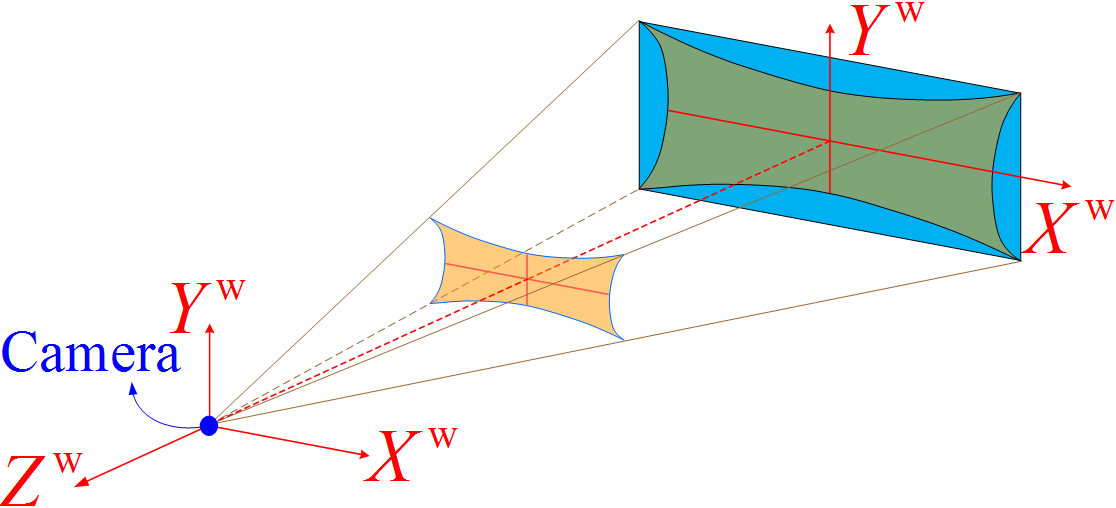
\includegraphics[width=\textwidth]{CaliPinHolCameraModel}
%\caption{Lens Distortion Removed Pinhole Camera model}
%\label{CaliPinHolCameraModel}
%\end{figure}%
%%
%
%With \(X^w\)/\(Y^w\)'s lens distortions removed, the last thing to go for is to calculate beam equations for every single pixel. It is straight forward to determine a line equation (beam equation) given two know points. The first point is the origin, and the second point could be calculated using the high order transformation matrix.
%%%%%%%%%%%%%%
%%%%%%%%%%%%%%
%%%%%%%%%%%%%%
%%%%%%%%%%%%%%
%\subsection{Extended Method Two}
%The extended method one, which is introduced above, is still not ideal. The focal point and focal length of a camera practically will change as its lens changes, so that light rays should not converge at the origin, and probably not even at one point. In order to get more accurate LUT for a better 3D view, the second point of the beam for every single pixel should also be a datum retrieved from the camera. %
%%\\\\%
%The second method, chasing after accuracy, is to add a rail along \(Z^w\)-axis for multiple points data acquisition. Not only real points (in contrast to assuming the origin as the second point) will be used for beam equation determination, but the \(Z^w\) values could also be calibrated with external accurate data support in case \(depth\) distortion (as shown in fig.~\ref{NIR_by_Depth_LeftSide}).
%%
%\begin{figure}[H]
%\centering
%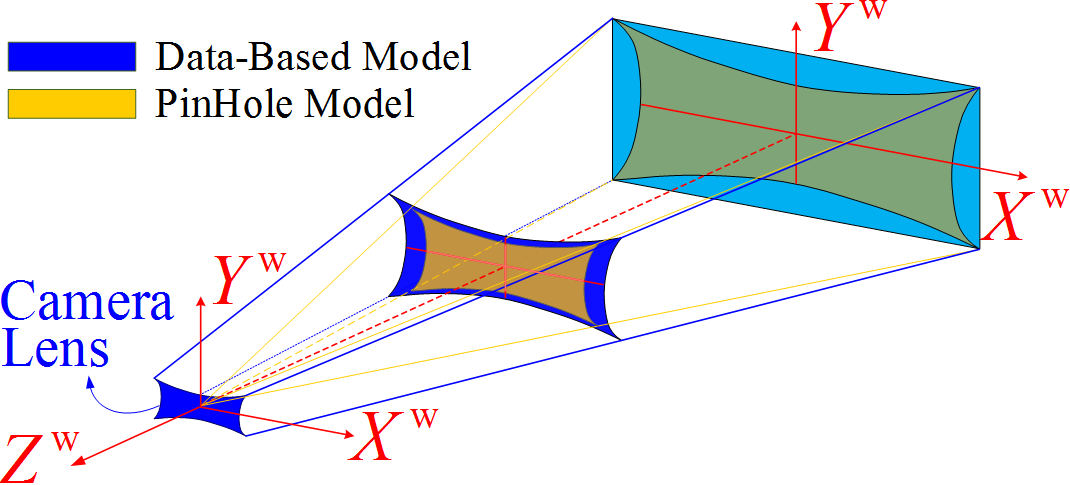
\includegraphics[width=\textwidth]{DataBasedCalibrationModel}
%\caption{Comparison: Data-Based Calibration and Pinhole Model Calibration}
%\label{DataBasedCalibrationModel}
%\end{figure}%
%%
%%
%
%fig.~\ref{DataBasedCalibrationModel} gives the data-based model in dark blue, whereas the pinhole camera model in yellow. Due to the fact that, the lens prolongs the focal length, the light rays after lens-distortion removed will converge in front of the origin instead of at the origin. The virtual converging point, which in pinhole camera model was at the origin, is now between the origin and the view, notes as \enquote{Virtual Camera Lens}. This model is proved practically on KinectV2 in section \ref{finalDataBasedModelReconstruction} fig.~\ref{SampleBeams_NearIR}.
%

























